% Options for packages loaded elsewhere
% Options for packages loaded elsewhere
\PassOptionsToPackage{unicode}{hyperref}
\PassOptionsToPackage{hyphens}{url}
\PassOptionsToPackage{dvipsnames,svgnames,x11names}{xcolor}
%
\documentclass[
  english,
  11pt,
  a4paper,
]{scrbook}
\usepackage{xcolor}
\usepackage[top=30mm,left=25mm,right=25mm,bottom=30mm]{geometry}
\usepackage{amsmath,amssymb}
\setcounter{secnumdepth}{5}
\usepackage{iftex}
\ifPDFTeX
  \usepackage[T1]{fontenc}
  \usepackage[utf8]{inputenc}
  \usepackage{textcomp} % provide euro and other symbols
\else % if luatex or xetex
  \usepackage{unicode-math} % this also loads fontspec
  \defaultfontfeatures{Scale=MatchLowercase}
  \defaultfontfeatures[\rmfamily]{Ligatures=TeX,Scale=1}
\fi
\usepackage{lmodern}
\ifPDFTeX\else
  % xetex/luatex font selection
\fi
% Use upquote if available, for straight quotes in verbatim environments
\IfFileExists{upquote.sty}{\usepackage{upquote}}{}
\IfFileExists{microtype.sty}{% use microtype if available
  \usepackage[]{microtype}
  \UseMicrotypeSet[protrusion]{basicmath} % disable protrusion for tt fonts
}{}
\makeatletter
\@ifundefined{KOMAClassName}{% if non-KOMA class
  \IfFileExists{parskip.sty}{%
    \usepackage{parskip}
  }{% else
    \setlength{\parindent}{0pt}
    \setlength{\parskip}{6pt plus 2pt minus 1pt}}
}{% if KOMA class
  \KOMAoptions{parskip=half}}
\makeatother
% Make \paragraph and \subparagraph free-standing
\makeatletter
\ifx\paragraph\undefined\else
  \let\oldparagraph\paragraph
  \renewcommand{\paragraph}{
    \@ifstar
      \xxxParagraphStar
      \xxxParagraphNoStar
  }
  \newcommand{\xxxParagraphStar}[1]{\oldparagraph*{#1}\mbox{}}
  \newcommand{\xxxParagraphNoStar}[1]{\oldparagraph{#1}\mbox{}}
\fi
\ifx\subparagraph\undefined\else
  \let\oldsubparagraph\subparagraph
  \renewcommand{\subparagraph}{
    \@ifstar
      \xxxSubParagraphStar
      \xxxSubParagraphNoStar
  }
  \newcommand{\xxxSubParagraphStar}[1]{\oldsubparagraph*{#1}\mbox{}}
  \newcommand{\xxxSubParagraphNoStar}[1]{\oldsubparagraph{#1}\mbox{}}
\fi
\makeatother


\usepackage{longtable,booktabs,array}
\newcounter{none} % for unnumbered tables
\usepackage{calc} % for calculating minipage widths
% Correct order of tables after \paragraph or \subparagraph
\usepackage{etoolbox}
\makeatletter
\patchcmd\longtable{\par}{\if@noskipsec\mbox{}\fi\par}{}{}
\makeatother
% Allow footnotes in longtable head/foot
\IfFileExists{footnotehyper.sty}{\usepackage{footnotehyper}}{\usepackage{footnote}}
\makesavenoteenv{longtable}
\usepackage{graphicx}
\makeatletter
\newsavebox\pandoc@box
\newcommand*\pandocbounded[1]{% scales image to fit in text height/width
  \sbox\pandoc@box{#1}%
  \Gscale@div\@tempa{\textheight}{\dimexpr\ht\pandoc@box+\dp\pandoc@box\relax}%
  \Gscale@div\@tempb{\linewidth}{\wd\pandoc@box}%
  \ifdim\@tempb\p@<\@tempa\p@\let\@tempa\@tempb\fi% select the smaller of both
  \ifdim\@tempa\p@<\p@\scalebox{\@tempa}{\usebox\pandoc@box}%
  \else\usebox{\pandoc@box}%
  \fi%
}
% Set default figure placement to htbp
\def\fps@figure{htbp}
\makeatother


% definitions for citeproc citations
\NewDocumentCommand\citeproctext{}{}
\NewDocumentCommand\citeproc{mm}{%
  \begingroup\def\citeproctext{#2}\cite{#1}\endgroup}
\makeatletter
 % allow citations to break across lines
 \let\@cite@ofmt\@firstofone
 % avoid brackets around text for \cite:
 \def\@biblabel#1{}
 \def\@cite#1#2{{#1\if@tempswa , #2\fi}}
\makeatother
\newlength{\cslhangindent}
\setlength{\cslhangindent}{1.5em}
\newlength{\csllabelwidth}
\setlength{\csllabelwidth}{3em}
\newenvironment{CSLReferences}[2] % #1 hanging-indent, #2 entry-spacing
 {\begin{list}{}{%
  \setlength{\itemindent}{0pt}
  \setlength{\leftmargin}{0pt}
  \setlength{\parsep}{0pt}
  % turn on hanging indent if param 1 is 1
  \ifodd #1
   \setlength{\leftmargin}{\cslhangindent}
   \setlength{\itemindent}{-1\cslhangindent}
  \fi
  % set entry spacing
  \setlength{\itemsep}{#2\baselineskip}}}
 {\end{list}}
\usepackage{calc}
\newcommand{\CSLBlock}[1]{\hfill\break\parbox[t]{\linewidth}{\strut\ignorespaces#1\strut}}
\newcommand{\CSLLeftMargin}[1]{\parbox[t]{\csllabelwidth}{\strut#1\strut}}
\newcommand{\CSLRightInline}[1]{\parbox[t]{\linewidth - \csllabelwidth}{\strut#1\strut}}
\newcommand{\CSLIndent}[1]{\hspace{\cslhangindent}#1}

\ifLuaTeX
\usepackage[bidi=basic,shorthands=off]{babel}
\else
\usepackage[bidi=default,shorthands=off]{babel}
\fi
\ifLuaTeX
  \usepackage{selnolig} % disable illegal ligatures
\fi


\setlength{\emergencystretch}{3em} % prevent overfull lines

\providecommand{\tightlist}{%
  \setlength{\itemsep}{0pt}\setlength{\parskip}{0pt}}



 


\makeatletter
\@ifpackageloaded{tcolorbox}{}{\usepackage[skins,breakable]{tcolorbox}}
\@ifpackageloaded{fontawesome5}{}{\usepackage{fontawesome5}}
\definecolor{quarto-callout-color}{HTML}{909090}
\definecolor{quarto-callout-note-color}{HTML}{0758E5}
\definecolor{quarto-callout-important-color}{HTML}{CC1914}
\definecolor{quarto-callout-warning-color}{HTML}{EB9113}
\definecolor{quarto-callout-tip-color}{HTML}{00A047}
\definecolor{quarto-callout-caution-color}{HTML}{FC5300}
\definecolor{quarto-callout-color-frame}{HTML}{acacac}
\definecolor{quarto-callout-note-color-frame}{HTML}{4582ec}
\definecolor{quarto-callout-important-color-frame}{HTML}{d9534f}
\definecolor{quarto-callout-warning-color-frame}{HTML}{f0ad4e}
\definecolor{quarto-callout-tip-color-frame}{HTML}{02b875}
\definecolor{quarto-callout-caution-color-frame}{HTML}{fd7e14}
\makeatother
\makeatletter
\@ifpackageloaded{bookmark}{}{\usepackage{bookmark}}
\makeatother
\makeatletter
\@ifpackageloaded{caption}{}{\usepackage{caption}}
\AtBeginDocument{%
\ifdefined\contentsname
  \renewcommand*\contentsname{Table of contents}
\else
  \newcommand\contentsname{Table of contents}
\fi
\ifdefined\listfigurename
  \renewcommand*\listfigurename{List of Figures}
\else
  \newcommand\listfigurename{List of Figures}
\fi
\ifdefined\listtablename
  \renewcommand*\listtablename{List of Tables}
\else
  \newcommand\listtablename{List of Tables}
\fi
\ifdefined\figurename
  \renewcommand*\figurename{Figure}
\else
  \newcommand\figurename{Figure}
\fi
\ifdefined\tablename
  \renewcommand*\tablename{Table}
\else
  \newcommand\tablename{Table}
\fi
}
\@ifpackageloaded{float}{}{\usepackage{float}}
\floatstyle{ruled}
\@ifundefined{c@chapter}{\newfloat{codelisting}{h}{lop}}{\newfloat{codelisting}{h}{lop}[chapter]}
\floatname{codelisting}{Listing}
\newcommand*\listoflistings{\listof{codelisting}{List of Listings}}
\makeatother
\makeatletter
\makeatother
\makeatletter
\@ifpackageloaded{caption}{}{\usepackage{caption}}
\@ifpackageloaded{subcaption}{}{\usepackage{subcaption}}
\makeatother
\usepackage{bookmark}
\IfFileExists{xurl.sty}{\usepackage{xurl}}{} % add URL line breaks if available
\urlstyle{same}
\hypersetup{
  pdftitle={The BPA Lab},
  pdfauthor={Matthias Zapp},
  pdflang={en},
  colorlinks=true,
  linkcolor={Maroon},
  filecolor={Maroon},
  citecolor={Blue},
  urlcolor={Blue},
  pdfcreator={LaTeX via pandoc}}


\title{The BPA Lab}
\usepackage{etoolbox}
\makeatletter
\providecommand{\subtitle}[1]{% add subtitle to \maketitle
  \apptocmd{\@title}{\par {\large #1 \par}}{}{}
}
\makeatother
\subtitle{Architecture and Documentation of a Demonstration Factory for
Business Process Automation and Analytics}
\author{Matthias Zapp}
\date{May 22, 2026}
\begin{document}
\frontmatter
\maketitle

\renewcommand*\contentsname{Table of contents}
{
\setcounter{tocdepth}{2}
\tableofcontents
}

\mainmatter
\bookmarksetup{startatroot}

\chapter{Overview}\label{overview}

\begin{figure}

\centering{

\pandocbounded{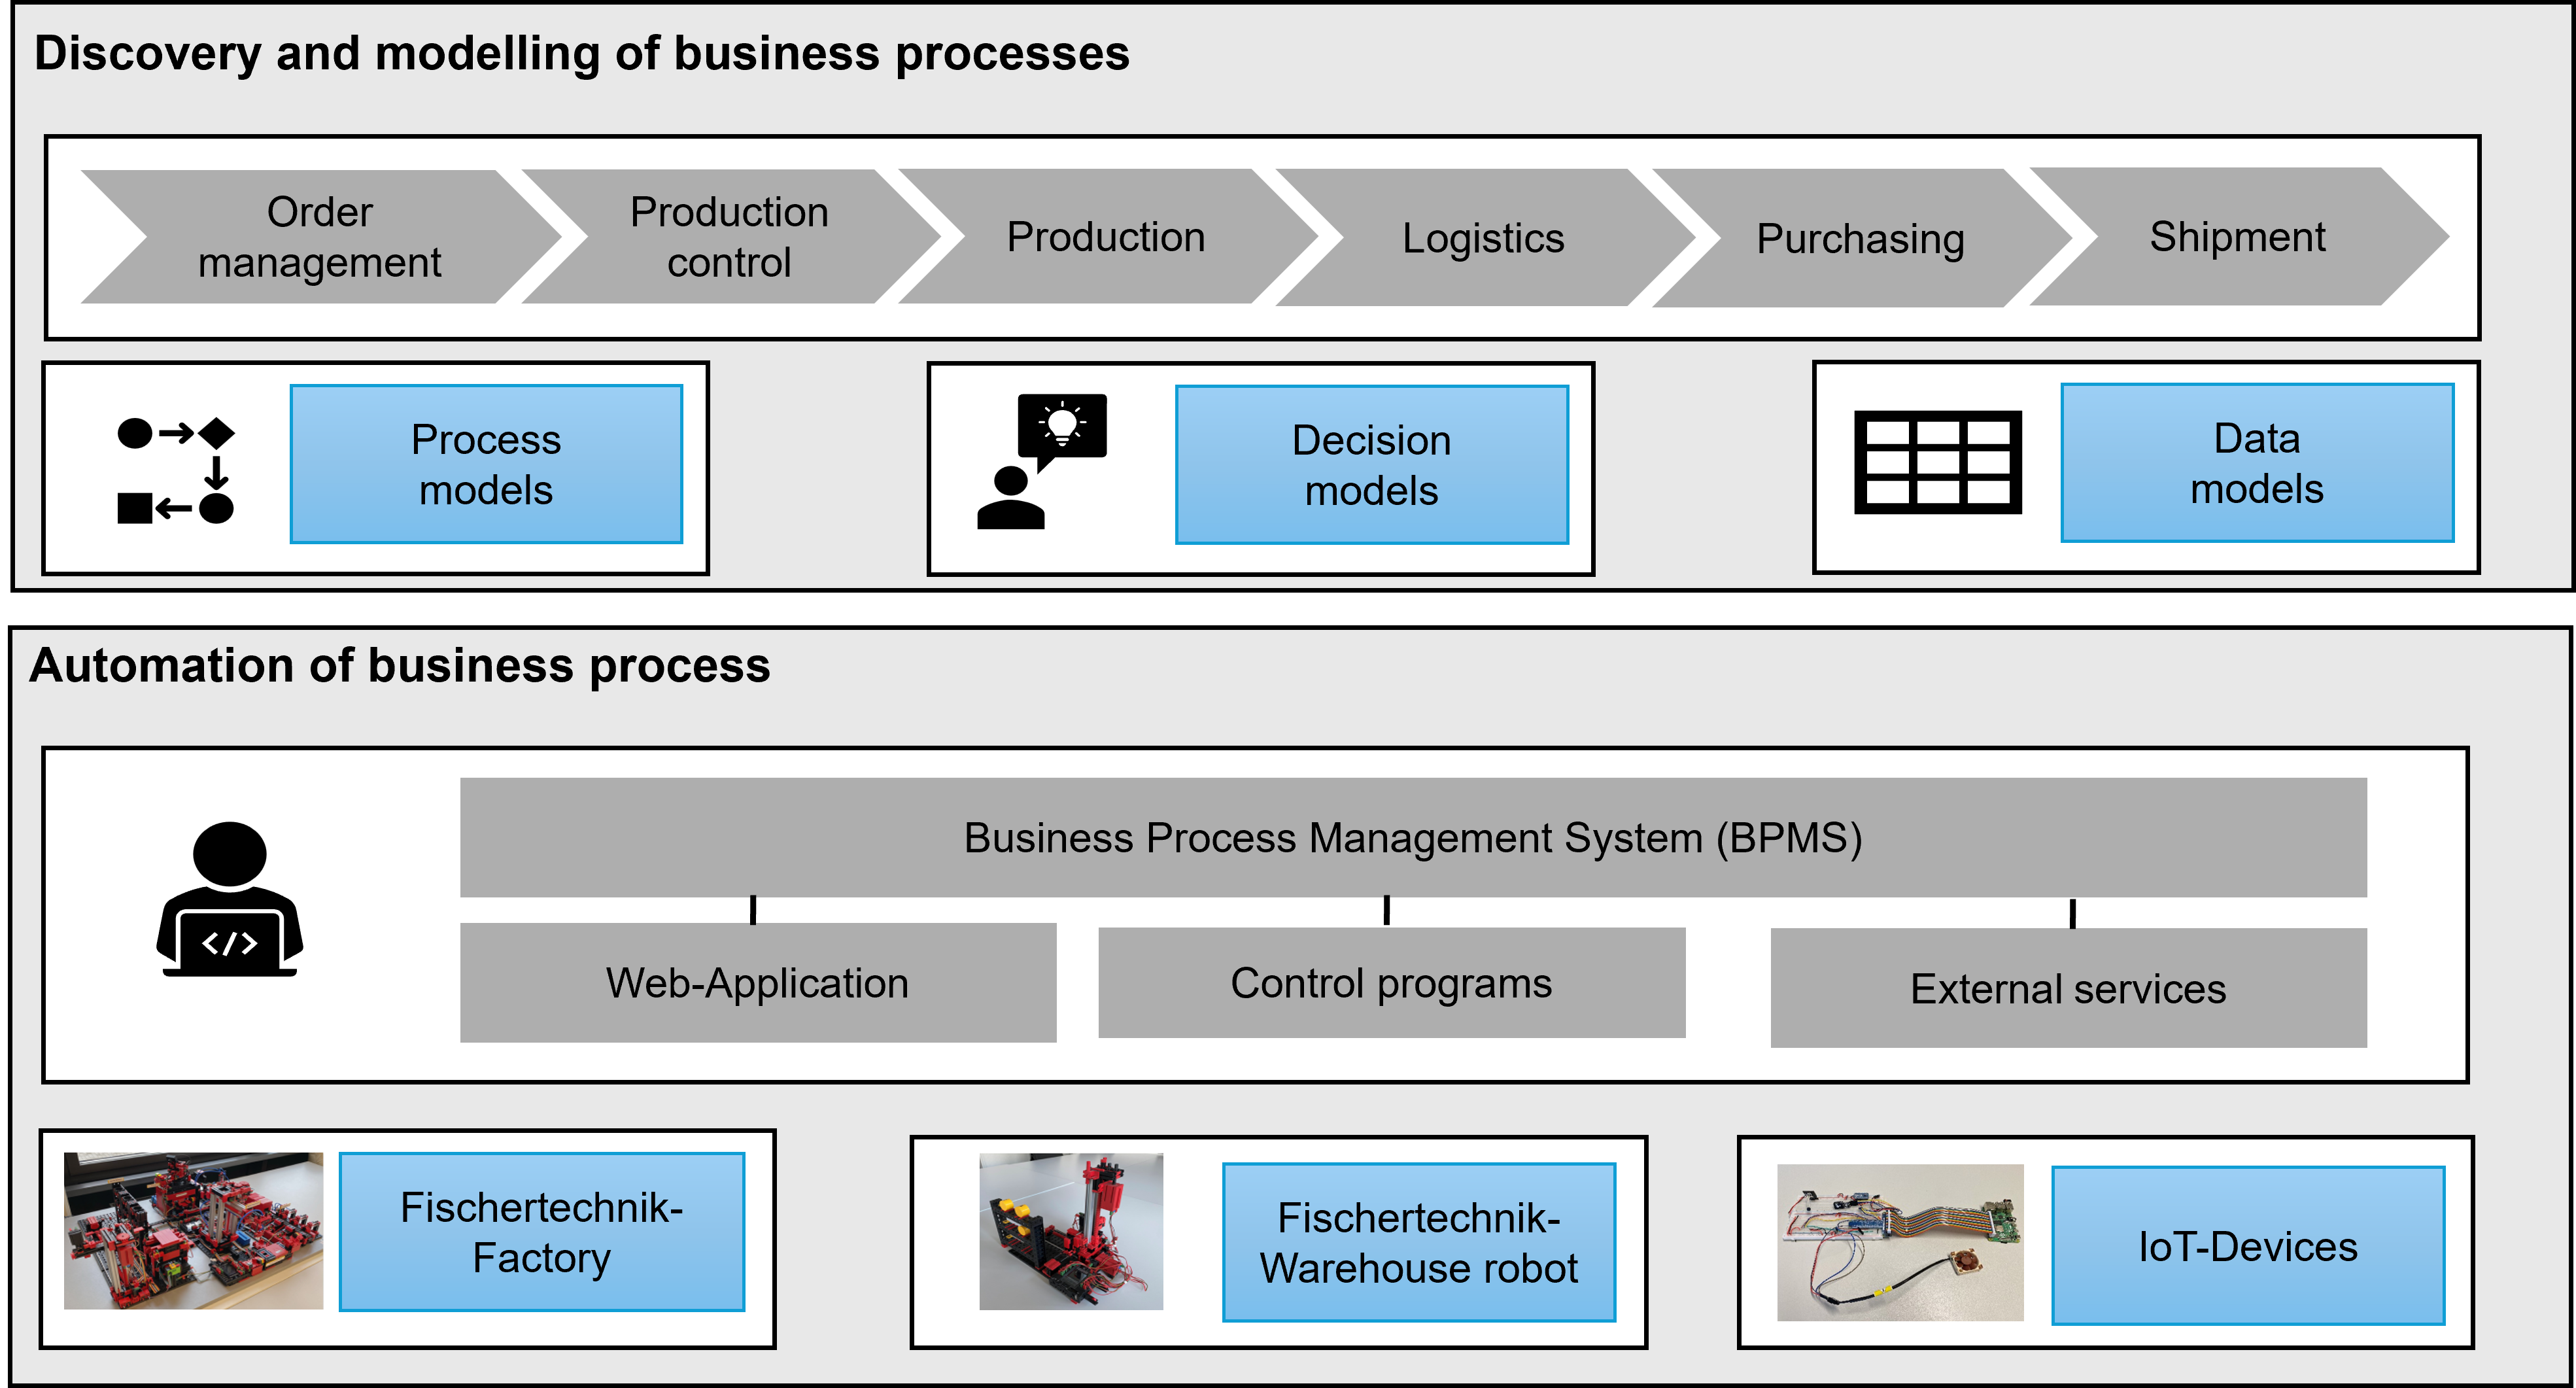
\includegraphics[keepaspectratio]{images/Conceptional_Architecture.png}}

}

\caption{\label{fig-concept}BPA Lab --- Conceptual Architecture}

\end{figure}%

This book documents the \textbf{Business Process Automation Lab (BPA
Lab)} at TH Köln --- a small-scale, modular model factory that
demonstrates and teaches concepts and technologies for business process
automation and analytics.

\section{About this book}\label{about-this-book}

The BPA Lab combines \textbf{software components} (Business Process
Management Systems, Robotic Process Automation, Process Mining) with
\textbf{hardware components} (a Fischertechnik Industry 4.0 factory, a
Fischertechnik warehouse robot, and IoT devices) to simulate the
production and logistics processes of a bicycle manufacturer.

This book aims to provide:

\begin{enumerate}
\def\labelenumi{\arabic{enumi}.}
\tightlist
\item
  A \textbf{high-level overview} of the BPA Lab and its goals.
\item
  A \textbf{description of the business scenario} --- the end-to-end
  ordering, manufacturing, and shipment process implemented in the lab.
\item
  A \textbf{description of the software architecture} and the design
  decisions taken along the way.
\end{enumerate}

It is structured as follows:

\begin{enumerate}
\def\labelenumi{\arabic{enumi}.}
\tightlist
\item
  \textbf{Introduction:} Motivation, goals, and scope of the BPA Lab.
\item
  \textbf{Solution overview:} The three architectural layers ---
  controllers, process applications, workflow engine.
\item
  \textbf{Business scenario:} The end-to-end bicycle ordering,
  manufacturing, and shipment process, broken down into its
  sub-processes (order management, production control, purchasing,
  manufacturing, shipment, warehouse operations).
\item
  \textbf{Data and data sources:} Data model, data flows, and
  persistence in the BPA Lab.
\item
  \textbf{Software architecture:} Requirements and a C4 view of the
  system.
\item
  \textbf{Architecture decisions:} Documented decisions and their
  rationales.
\end{enumerate}

The appendices contain:

\begin{itemize}
\tightlist
\item
  \textbf{Appendix A:} Overview of related components and sister
  repositories.
\item
  \textbf{Appendix B:} A glossary of key terms.
\item
  \textbf{References:} All cited literature.
\end{itemize}

\section{Who this book is for}\label{who-this-book-is-for}

This book is written for:

\begin{itemize}
\tightlist
\item
  \textbf{Lecturers and researchers} who want to teach business process
  automation with a tangible, end-to-end reference system.
\item
  \textbf{Students} working on bachelor's or master's projects inside
  the BPA Lab.
\item
  \textbf{Practitioners} looking for a concrete reference architecture
  combining a BPMS, IoT hardware, and process mining.
\end{itemize}

\section{Source code and related
repositories}\label{source-code-and-related-repositories}

The implementation of the demonstration factory is maintained as a
separate repository:
\href{https://github.com/BpaLabTHCologne/bpa_lab_demonstration_factory}{bpa\_lab\_demonstration\_factory}.

Documentation for student component projects is available in the wiki of
\href{https://github.com/BpaLabTHCologne/bpa_lab_student_docs/wiki}{bpa\_lab\_student\_docs}.

\section{Status and roadmap}\label{status-and-roadmap}

\begin{tcolorbox}[enhanced jigsaw, arc=.35mm, bottomrule=.15mm, bottomtitle=1mm, breakable, colback=white, colbacktitle=quarto-callout-important-color!10!white, colframe=quarto-callout-important-color-frame, coltitle=black, left=2mm, leftrule=.75mm, opacityback=0, opacitybacktitle=0.6, rightrule=.15mm, title=\textcolor{quarto-callout-important-color}{\faExclamation}\hspace{0.5em}{Work in progress}, titlerule=0mm, toprule=.15mm, toptitle=1mm]

The BPA Lab --- and this book --- are under continuous development.
Several sections are marked as \emph{work in progress} and will be
expanded in future revisions. Bug reports and suggestions are very
welcome via the
\href{https://github.com/BpaLabTHCologne/bpa_lab_book/issues}{issue
tracker}.

\end{tcolorbox}

\section{Licence and citation}\label{licence-and-citation}

This work is published under the \textbf{Creative Commons
Attribution-ShareAlike 4.0} licence (CC BY-SA 4.0).

Suggested citation:

\begin{quote}
Zapp, Matthias (2026). \emph{The BPA Lab --- Architecture and
Documentation of a Demonstration Factory for Business Process Automation
and Analytics.} TH Köln (University of Applied Sciences). Online:
\url{https://bpalabthcologne.github.io/bpa_lab_book/}.
\end{quote}

\bookmarksetup{startatroot}

\chapter{Introduction}\label{introduction}

\begin{tcolorbox}[enhanced jigsaw, arc=.35mm, bottomrule=.15mm, bottomtitle=1mm, breakable, colback=white, colbacktitle=quarto-callout-note-color!10!white, colframe=quarto-callout-note-color-frame, coltitle=black, left=2mm, leftrule=.75mm, opacityback=0, opacitybacktitle=0.6, rightrule=.15mm, title=\textcolor{quarto-callout-note-color}{\faInfo}\hspace{0.5em}{Learning objectives}, titlerule=0mm, toprule=.15mm, toptitle=1mm]

After reading this chapter, you will be able to:

\begin{itemize}
\tightlist
\item
  describe the purpose and main goals of the BPA Lab,
\item
  distinguish between its \emph{demonstration} and \emph{teaching}
  missions,
\item
  identify the main hardware and software components and their roles.
\end{itemize}

\end{tcolorbox}

\section{What is the BPA Lab?}\label{what-is-the-bpa-lab}

The \textbf{Business Process Automation Lab (BPA Lab)} at TH Köln is a
small, modular model factory dedicated to business process automation
and analytics. It combines real-world software components used in
industry --- Business Process Management Systems (BPMS), Robotic Process
Automation (RPA), and process-mining tools --- with physical hardware: a
Fischertechnik Industry 4.0 factory, a Fischertechnik warehouse robot,
and a range of IoT devices.

Together, these components simulate the \textbf{production and logistics
processes of a bicycle manufacturer} --- from the customer order to the
delivery of a custom-built bike.

\section{Two goals: demonstration and
teaching}\label{two-goals-demonstration-and-teaching}

The BPA Lab pursues two complementary goals.

\subsection{Demonstration}\label{demonstration}

The lab demonstrates concepts and technologies for business process
automation and analytics in a tangible way. It shows how:

\begin{itemize}
\tightlist
\item
  a central BPMS (Camunda 8) orchestrates end-to-end business processes,
\item
  modular \textbf{job workers} implement the actual work and interact
  with hardware,
\item
  \textbf{process mining} can be used to analyse process executions and
  identify improvement opportunities.
\end{itemize}

By bringing together software and hardware in one running system, the
lab makes abstract concepts immediately visible.

\subsection{Teaching}\label{teaching}

Individual building blocks of the BPA Lab --- for instance the
Fischertechnik warehouse robot --- are also used in \textbf{student
projects} (bachelor's and master's level) as starting points for
self-defined process implementations. This enables a hands-on form of
teaching for \textbf{process-oriented application integration}: students
do not merely model processes on paper but see them execute in a real,
physical system.

\section{Why a demonstration
factory?}\label{why-a-demonstration-factory}

Business process management theory and notations like BPMN are often
taught using abstract examples --- pizza ordering, expense approvals,
generic procurement workflows. These examples are accessible but rarely
convey:

\begin{itemize}
\tightlist
\item
  the \textbf{technical complexity} of integrating heterogeneous
  systems,
\item
  the \textbf{operational concerns} of running long-lived process
  instances,
\item
  the \textbf{data perspective} that is at the heart of process mining
  and analytics.
\end{itemize}

A demonstration factory bridges this gap. Students and visitors can
observe how a customer order arrives via a web form, triggers a workflow
in Camunda 8, dispatches commands via MQTT to physical hardware, and
eventually leads to a real, manufactured product being moved through a
real, physical warehouse.

\section{A bird's-eye view}\label{a-birds-eye-view}

The next chapter --- \href{chapter02-solution-overview.qmd}{Solution
overview} --- introduces the three architectural layers of the BPA Lab.
Subsequent chapters describe the business scenario, the data
perspective, the software architecture, and the architecture decisions
taken so far.

\begin{tcolorbox}[enhanced jigsaw, arc=.35mm, bottomrule=.15mm, bottomtitle=1mm, breakable, colback=white, colbacktitle=quarto-callout-tip-color!10!white, colframe=quarto-callout-tip-color-frame, coltitle=black, left=2mm, leftrule=.75mm, opacityback=0, opacitybacktitle=0.6, rightrule=.15mm, title=\textcolor{quarto-callout-tip-color}{\faLightbulb}\hspace{0.5em}{How to read this book}, titlerule=0mm, toprule=.15mm, toptitle=1mm]

If you are new to the BPA Lab, read the chapters in order. If you are
already familiar with the lab and want to consult a specific aspect ---
for example a particular sub-process or an architectural decision ---
feel free to jump directly to the relevant chapter using the sidebar or
the search box at the top of the page.

\end{tcolorbox}

\bookmarksetup{startatroot}

\chapter{Solution Overview}\label{solution-overview}

\begin{tcolorbox}[enhanced jigsaw, arc=.35mm, bottomrule=.15mm, bottomtitle=1mm, breakable, colback=white, colbacktitle=quarto-callout-note-color!10!white, colframe=quarto-callout-note-color-frame, coltitle=black, left=2mm, leftrule=.75mm, opacityback=0, opacitybacktitle=0.6, rightrule=.15mm, title=\textcolor{quarto-callout-note-color}{\faInfo}\hspace{0.5em}{Learning objectives}, titlerule=0mm, toprule=.15mm, toptitle=1mm]

After reading this chapter, you will be able to:

\begin{itemize}
\tightlist
\item
  name the three architectural layers of the BPA Lab and explain their
  responsibilities,
\item
  describe the role of Camunda 8 as the central workflow engine,
\item
  explain how hardware components and process applications interact,
\item
  justify the modular, domain-driven design approach used in the BPA
  Lab.
\end{itemize}

\end{tcolorbox}

\section{Three architectural layers}\label{three-architectural-layers}

The architecture and implementation of the BPA Lab are under continuous
development. The solution is structured into three clearly separated
layers.

\subsection{Layer 1 --- Controllers}\label{layer-1-controllers}

\textbf{Controllers} are responsible for the direct control of hardware
components: the Fischertechnik Industry 4.0 factory, the Fischertechnik
warehouse robots, and IoT devices. They are predominantly implemented in
\textbf{Python} and translate high-level commands (for example
\emph{``transport workpiece from slot A to slot B''}) into the low-level
signals that move motors and read sensors.

\subsection{Layer 2 --- Process applications (job
workers)}\label{layer-2-process-applications-job-workers}

\textbf{Process applications} are middleware components that implement
the actual business logic of individual work steps. In Camunda 8 terms,
they are \textbf{job workers}: they subscribe to specific service tasks
and execute them when activated by the workflow engine.

Job workers communicate:

\begin{itemize}
\tightlist
\item
  with the \textbf{workflow engine} via \textbf{gRPC} (the standard
  Camunda 8 / Zeebe protocol),
\item
  with the \textbf{controllers} via \textbf{MQTT} (a lightweight
  publish-subscribe protocol that is well established in the IoT space).
\end{itemize}

Process applications are predominantly implemented in \textbf{Java}.

\subsection{Layer 3 --- BPMS workflow
engine}\label{layer-3-bpms-workflow-engine}

The central workflow engine is \textbf{Camunda 8 (self-managed)}. It
executes:

\begin{itemize}
\tightlist
\item
  \textbf{BPMN} process models --- describing how work flows through the
  system,
\item
  \textbf{DMN} decision models --- encoding business rules.
\end{itemize}

Camunda 8 maintains the state of each running process instance, handles
incidents, and provides the data foundation for process mining and
analytics.

\section{A modular, domain-driven
design}\label{a-modular-domain-driven-design}

A key design principle in the BPA Lab is \textbf{modularity}. The system
follows a \textbf{Domain-Driven Design (DDD)} approach so that:

\begin{itemize}
\tightlist
\item
  \textbf{multiple students and developers can work in parallel} on
  different parts of the system without stepping on each other's toes,
\item
  \textbf{components can be reused} in student projects to build new
  process applications,
\item
  \textbf{components can be replaced or upgraded} independently.
\end{itemize}

The primary criterion for splitting job workers and process models is
the \textbf{business domain}:

\begin{itemize}
\tightlist
\item
  Order management
\item
  Manufacturing
\item
  Shipping
\item
  Purchasing
\item
  Logistics / warehouse operations
\end{itemize}

This separation aligns with the bounded contexts familiar from DDD and
makes the system easier to reason about, both for teachers explaining it
and for students extending it.

\section{A simplified bird's-eye
view}\label{a-simplified-birds-eye-view}

The following diagram summarises the interaction between the three
layers and the hardware they ultimately drive.

\begin{figure}

\centering{

\pandocbounded{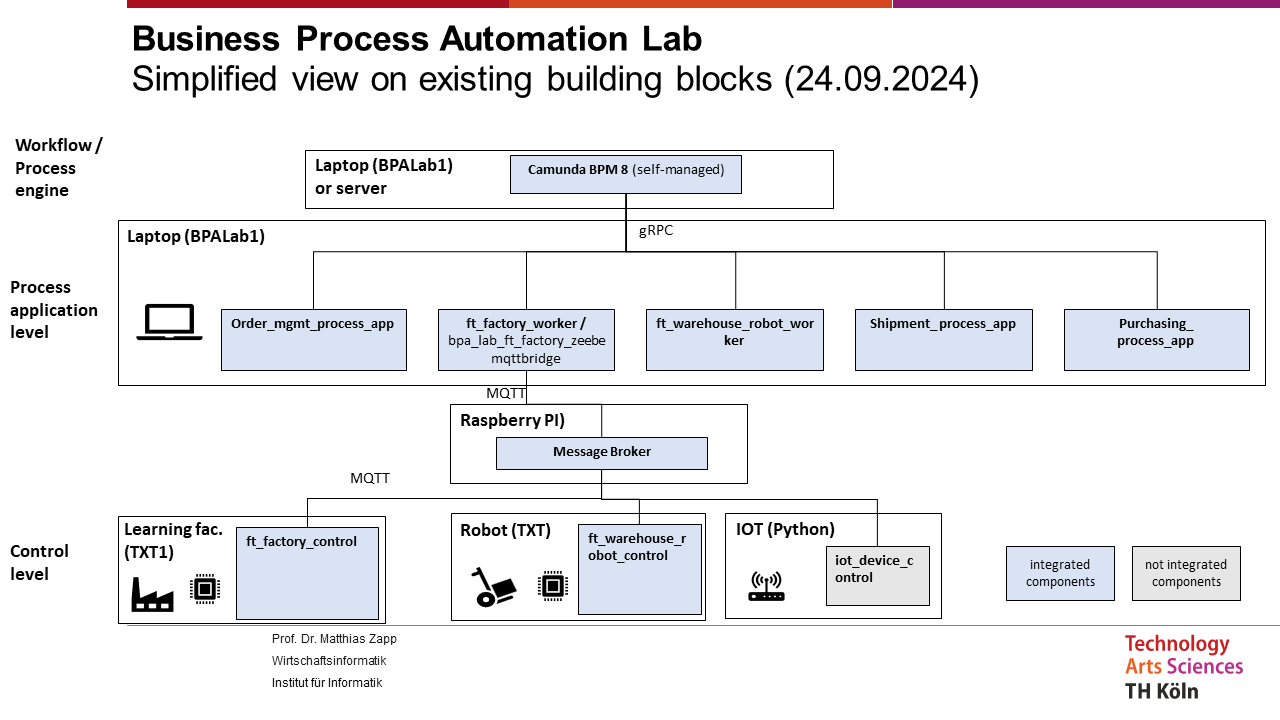
\includegraphics[keepaspectratio]{images/BPALab_Simplified_Arch_240924.png}}

}

\caption{\label{fig-simplified}Simplified architecture of the BPA Lab}

\end{figure}%

The customer-facing entry point is typically a \textbf{web application}
for order capture. From there, work flows downwards through Camunda 8
and the job workers and eventually reaches the physical Fischertechnik
components. Events generated along the way flow back upwards and are
persisted in databases for later analysis.

\section{The demonstration factory
implementation}\label{the-demonstration-factory-implementation}

The latest version of the BPA Lab as a runnable \textbf{demonstration
factory} is available in a separate repository:

➡️
\href{https://github.com/BpaLabTHCologne/bpa_lab_demonstration_factory}{github.com/BpaLabTHCologne/bpa\_lab\_demonstration\_factory}

The implementation is fully containerised with \textbf{Docker}. This
makes local setup straightforward and ensures that the environment is
reproducible across different machines --- a key requirement when
students set up the system on their own laptops.

\begin{tcolorbox}[enhanced jigsaw, arc=.35mm, bottomrule=.15mm, bottomtitle=1mm, breakable, colback=white, colbacktitle=quarto-callout-tip-color!10!white, colframe=quarto-callout-tip-color-frame, coltitle=black, left=2mm, leftrule=.75mm, opacityback=0, opacitybacktitle=0.6, rightrule=.15mm, title=\textcolor{quarto-callout-tip-color}{\faLightbulb}\hspace{0.5em}{Getting started in practice}, titlerule=0mm, toprule=.15mm, toptitle=1mm]

If you are setting up the BPA Lab for the first time, start with the
\texttt{docker-compose.yml} of the demonstration factory and follow the
installation guide there. To develop your own components on top of the
lab, the
\href{https://github.com/BpaLabTHCologne/bpa_lab_student_docs/wiki}{student-docs
wiki} provides component-level guides.

\end{tcolorbox}

\bookmarksetup{startatroot}

\chapter{Business Scenario of the Demonstration
Factory}\label{business-scenario-of-the-demonstration-factory}

\begin{tcolorbox}[enhanced jigsaw, arc=.35mm, bottomrule=.15mm, bottomtitle=1mm, breakable, colback=white, colbacktitle=quarto-callout-note-color!10!white, colframe=quarto-callout-note-color-frame, coltitle=black, left=2mm, leftrule=.75mm, opacityback=0, opacitybacktitle=0.6, rightrule=.15mm, title=\textcolor{quarto-callout-note-color}{\faInfo}\hspace{0.5em}{Learning objectives}, titlerule=0mm, toprule=.15mm, toptitle=1mm]

After reading this chapter, you will be able to:

\begin{itemize}
\tightlist
\item
  describe the end-to-end business processes of a custom bicycle
  manufacturer in BPMN terms,
\item
  explain the orchestrating role of the order management process,
\item
  distinguish between the responsibilities of the order management,
  production control, purchasing, manufacturing, shipment, and warehouse
  operations processes,
\item
  recognise how Fischertechnik hardware is used to \emph{physically}
  execute parts of these processes.
\end{itemize}

\end{tcolorbox}

\begin{tcolorbox}[enhanced jigsaw, arc=.35mm, bottomrule=.15mm, bottomtitle=1mm, breakable, colback=white, colbacktitle=quarto-callout-important-color!10!white, colframe=quarto-callout-important-color-frame, coltitle=black, left=2mm, leftrule=.75mm, opacityback=0, opacitybacktitle=0.6, rightrule=.15mm, title=\textcolor{quarto-callout-important-color}{\faExclamation}\hspace{0.5em}{Status of this chapter}, titlerule=0mm, toprule=.15mm, toptitle=1mm]

This chapter describes the business processes of the BPA Lab at a
strategic level. It is \emph{work in progress} --- terminology, level of
detail, and harmonisation of process models are being refined as the lab
evolves.

\end{tcolorbox}

\section{The scenario in a nutshell}\label{the-scenario-in-a-nutshell}

\textbf{A bicycle manufacturer offers highly customisable bicycles to
consumers.}

The entire end-to-end process is orchestrated by the \textbf{order
management process}, which in turn initiates purchasing, manufacturing,
and shipping processes as needed.

\begin{figure}

\centering{

\pandocbounded{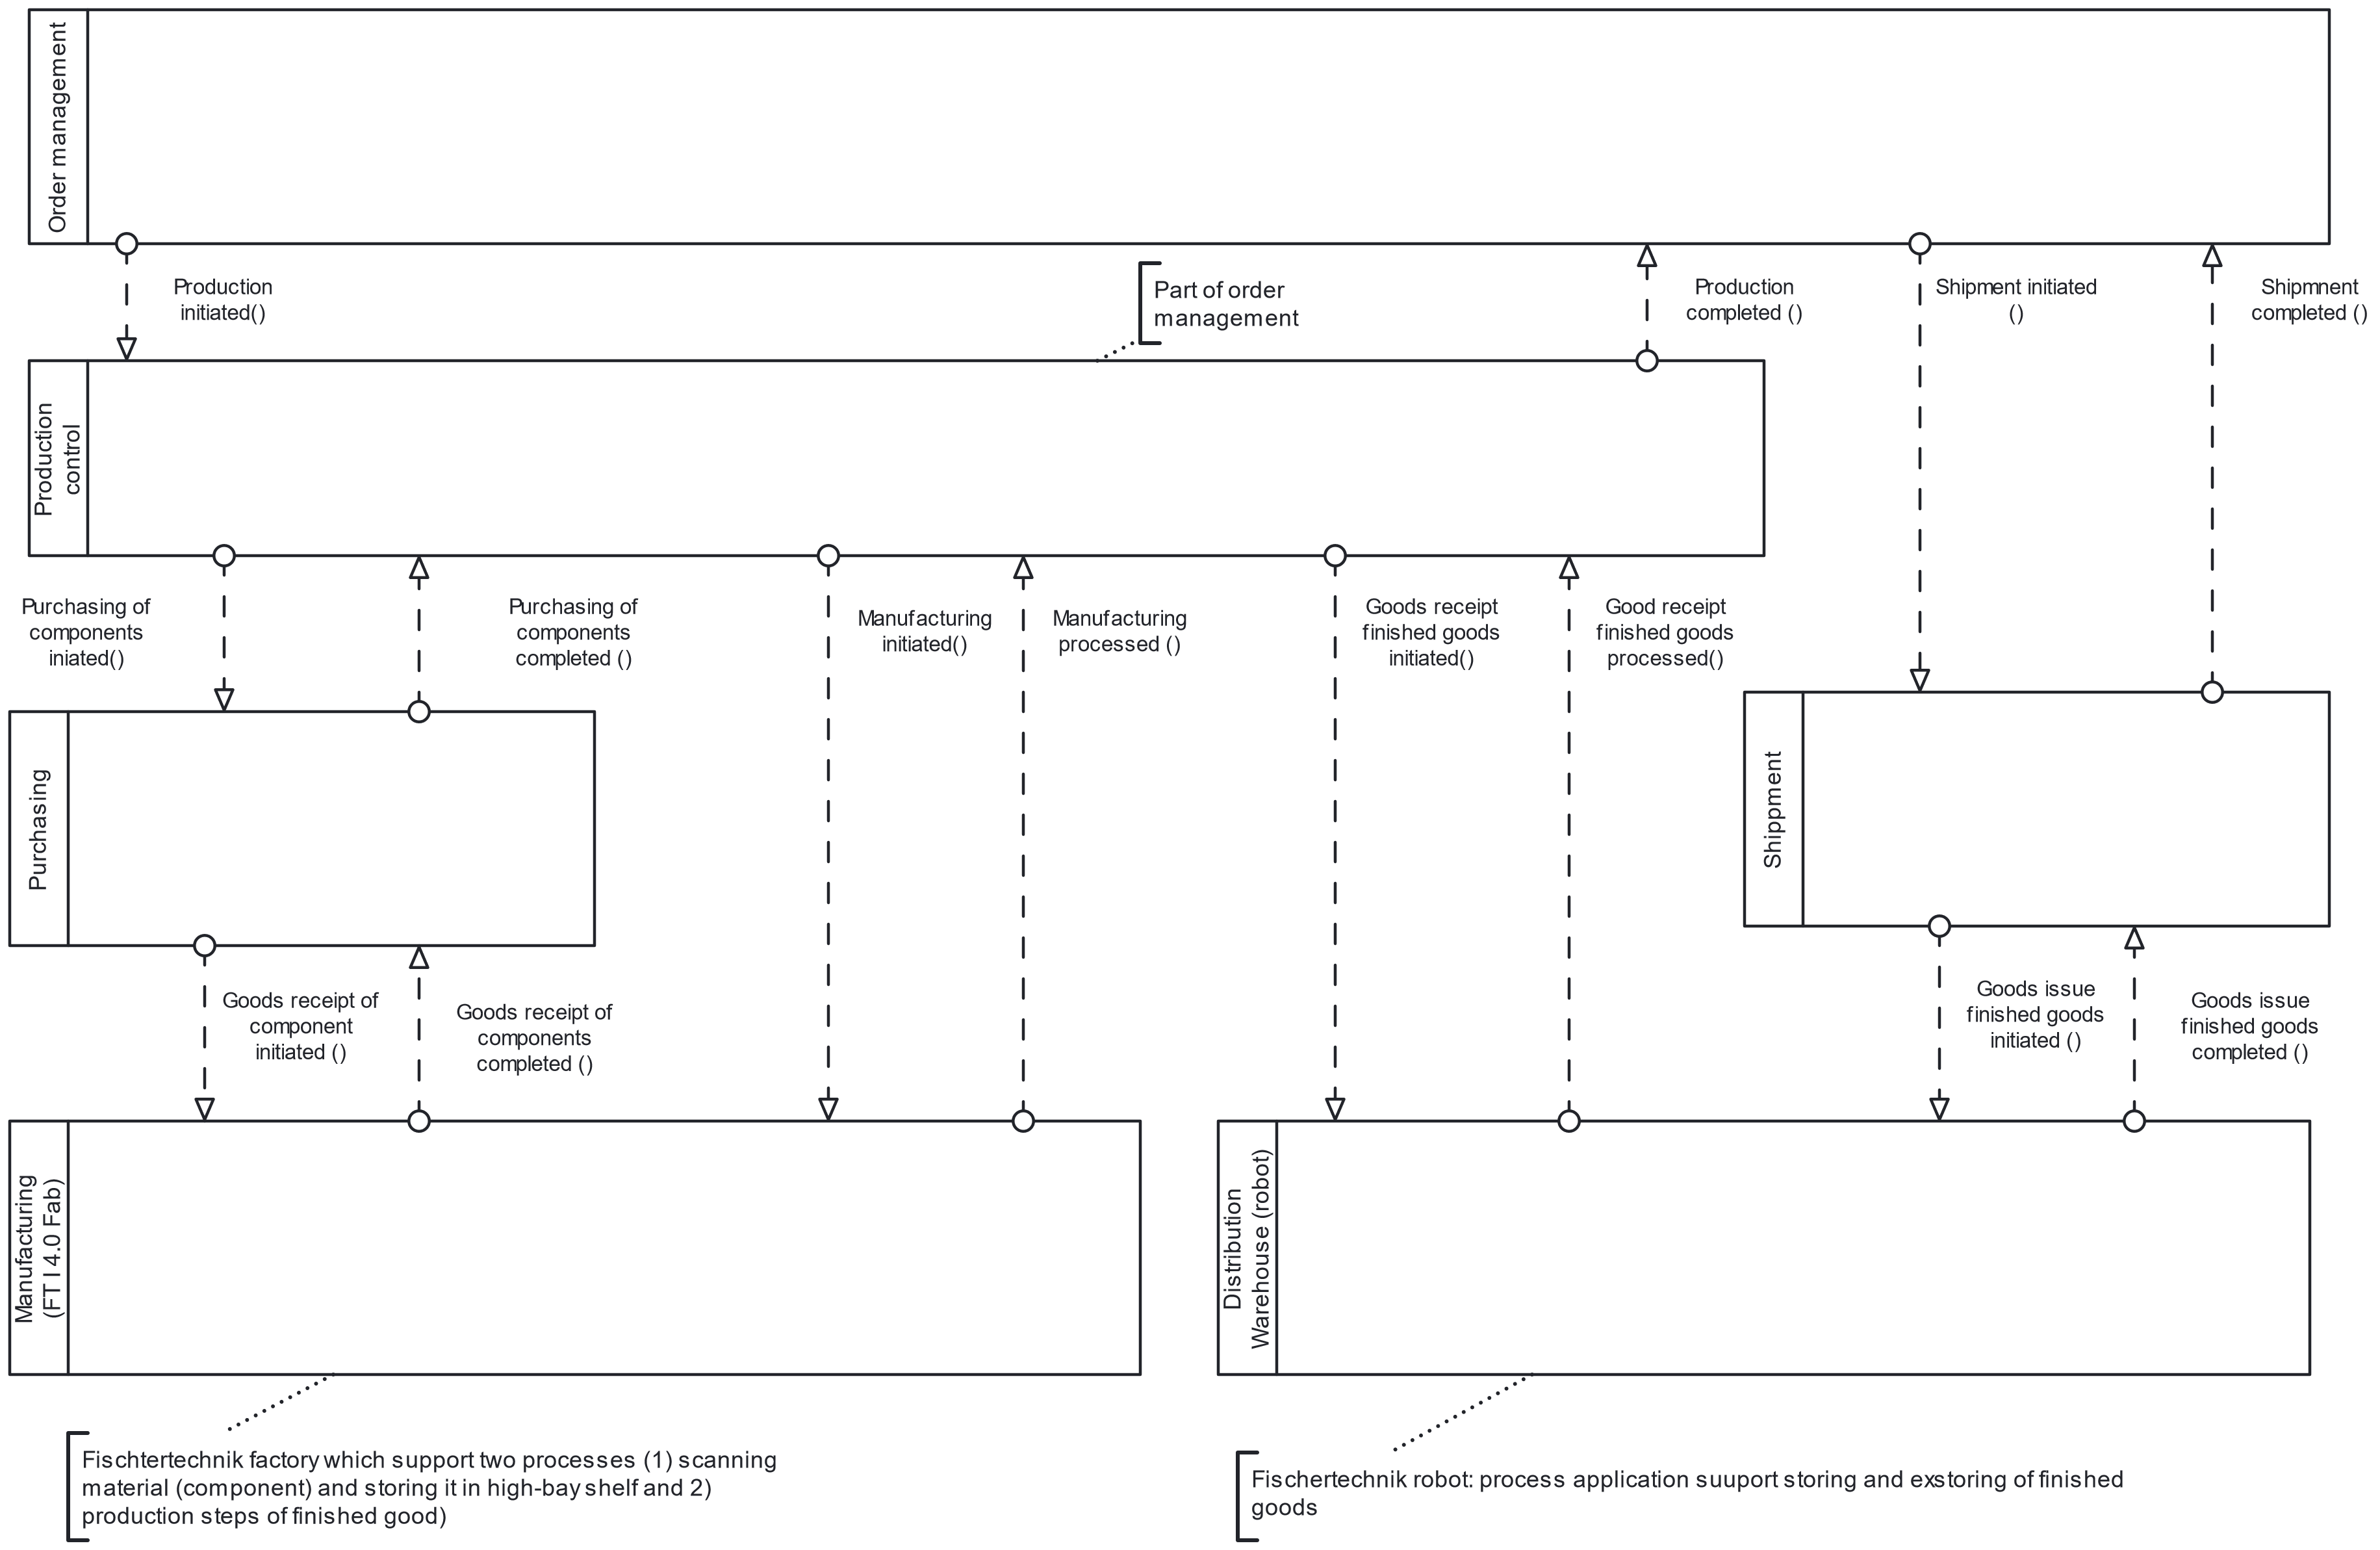
\includegraphics[keepaspectratio]{images/process_landscape.png}}

}

\caption{\label{fig-landscape}Process landscape of the BPA Lab}

\end{figure}%

The manufacturing processes use the \textbf{Fischertechnik Industry 4.0
factory} to post goods receipts of components and to perform the actual
manufacturing steps. Order management and shipping additionally use the
\textbf{distribution warehouse} (a separate Fischertechnik robot) to
post goods receipts and goods issues for finished products.

The following sections describe each sub-process in turn. The process
models do \textbf{not} include technical aspects and show only the
\textbf{happy path} of execution.

\section{Order management}\label{order-management}

\begin{figure}

\centering{

\pandocbounded{\includegraphics[keepaspectratio]{index_files/mediabag/BPALabBikeFactoryOrd.png}}

}

\caption{\label{fig-ordermgmt}Order management process}

\end{figure}%

The order management process governs the fulfilment of customer orders.

It starts when a customer order is entered into a web form, which is
pre-filled with product data (bicycle models) from the database. During
execution, the \textbf{availability of the ordered products} is checked.

Two main scenarios apply:

\begin{itemize}
\tightlist
\item
  \textbf{All products in stock:} the shipping process is triggered
  directly. Once shipping completes successfully, the process is
  finished.
\item
  \textbf{One or more products out of stock:} for each unavailable
  product, the production control process is triggered, which creates a
  \textbf{production order}. The production order specifies the required
  components.

  \begin{itemize}
  \tightlist
  \item
    If the components are also unavailable, a \textbf{purchasing
    process} is started first.
  \item
    Otherwise, the \textbf{manufacturing process} is triggered
    immediately.
  \end{itemize}
\end{itemize}

Once the missing products are manufactured, shipping is initiated.

\section{Production control}\label{production-control}

\begin{figure}

\centering{

\pandocbounded{\includegraphics[keepaspectratio]{index_files/mediabag/BPALabBikeFactoryPro.png}}

}

\caption{\label{fig-prodcontrol}Production control process}

\end{figure}%

The production control process manages the creation and execution of
\textbf{one production order for one product}. It determines the
component demand and --- if needed --- triggers a purchasing process to
procure the missing components. Once components are available, it
triggers the actual manufacturing process.

\section{Purchasing}\label{purchasing}

\begin{figure}

\centering{

\pandocbounded{\includegraphics[keepaspectratio]{index_files/mediabag/bpa_lab_purchase_pro.png}}

}

\caption{\label{fig-purchasing}Purchasing process}

\end{figure}%

The purchasing process manages the procurement of required components.
It starts whenever a component is needed and creates a \textbf{purchase
order}.

The purchase order can be adjusted by the user --- for example by
selecting a specific vendor. Materials are then stored and stock levels
are updated. Upon user confirmation (or after a configurable timeout),
the stock level is increased in the inventory database.

\section{Manufacturing}\label{manufacturing}

\begin{figure}

\centering{

\pandocbounded{\includegraphics[keepaspectratio]{index_files/mediabag/BPALabBikeFactoryMan.png}}

}

\caption{\label{fig-manufacturing}Manufacturing process}

\end{figure}%

The manufacturing process governs the \textbf{physical manufacturing
simulation} on the Fischertechnik factory for \textbf{one item of one
product type}.

It starts after a production order has been created by the production
control process and sufficient components are available.

The process must place a manufacturing order that produces a new bicycle
from the specified material. Before that, however, it must check whether
a \textbf{physical workpiece} is already available in the warehouse of
the Fischertechnik factory. If not, a physical workpiece must first be
transferred to the factory so that the control program can store and
recognise it. Once the bicycle has been produced from the material
(workpiece), the process is complete.

\section{Shipment}\label{shipment}

\begin{figure}

\centering{

\pandocbounded{\includegraphics[keepaspectratio]{index_files/mediabag/bpa_lab_shipment_pro.png}}

}

\caption{\label{fig-shipment}Shipment process}

\end{figure}%

The shipment process manages the dispatch of finished goods to the
customer. It is \textbf{only} triggered if a product is in stock and
ready to be shipped.

The flow is:

\begin{enumerate}
\def\labelenumi{\arabic{enumi}.}
\tightlist
\item
  Shipping data is checked.
\item
  The distance and duration from the warehouse to the delivery address
  are computed --- the \textbf{Openrouteservice API} is used for this.
\item
  The logistics sub-process retrieves the customer order from the
  warehouse.
\item
  A message is sent to the customer to inform them about the dispatch.
\item
  Upon handover of the order to the customer, both the shipping process
  and the surrounding end-to-end process instance are completed.
\end{enumerate}

\section{Warehouse operations}\label{warehouse-operations}

The warehouse operations process governs the flow of finished goods in a
distribution warehouse --- represented physically by the Fischertechnik
warehouse robot.

It starts when a \textbf{transfer order} for the warehouse is received
from another business process. A transfer order can be either an
instruction to \textbf{store products} in the warehouse or to
\textbf{retrieve products} from it.

\section{Teaching note}\label{teaching-note}

\begin{tcolorbox}[enhanced jigsaw, arc=.35mm, bottomrule=.15mm, bottomtitle=1mm, breakable, colback=white, colbacktitle=quarto-callout-tip-color!10!white, colframe=quarto-callout-tip-color-frame, coltitle=black, left=2mm, leftrule=.75mm, opacityback=0, opacitybacktitle=0.6, rightrule=.15mm, title=\textcolor{quarto-callout-tip-color}{\faLightbulb}\hspace{0.5em}{Process landscape as a teaching tool}, titlerule=0mm, toprule=.15mm, toptitle=1mm]

This process landscape works well to introduce key BPMN concepts in
context:

\begin{itemize}
\tightlist
\item
  \textbf{call activities} (e.g.~order management calling production
  control),
\item
  \textbf{message-based communication} between long-running processes,
\item
  \textbf{boundary events} to handle exceptions raised by job workers,
\item
  \textbf{multi-instance activities} for handling several products in a
  single order.
\end{itemize}

By stepping through the running system together with students, abstract
notation suddenly becomes concrete.

\end{tcolorbox}

\bookmarksetup{startatroot}

\chapter{Data and Data Sources}\label{data-and-data-sources}

\begin{tcolorbox}[enhanced jigsaw, arc=.35mm, bottomrule=.15mm, bottomtitle=1mm, breakable, colback=white, colbacktitle=quarto-callout-note-color!10!white, colframe=quarto-callout-note-color-frame, coltitle=black, left=2mm, leftrule=.75mm, opacityback=0, opacitybacktitle=0.6, rightrule=.15mm, title=\textcolor{quarto-callout-note-color}{\faInfo}\hspace{0.5em}{Learning objectives}, titlerule=0mm, toprule=.15mm, toptitle=1mm]

After reading this chapter, you will be able to:

\begin{itemize}
\tightlist
\item
  identify the main data sources in the BPA Lab,
\item
  describe the role of the relational database in the overall
  architecture,
\item
  explain how process and event data become the foundation for process
  mining.
\end{itemize}

\end{tcolorbox}

\section{Overview of data sources}\label{overview-of-data-sources}

The BPA Lab integrates data from several sources --- from \textbf{master
data} in a relational database, via \textbf{process state} maintained by
the workflow engine, to \textbf{sensor and telemetry data} from the
Fischertechnik components.

The following figure gives an overview of the main data sources and the
kinds of data they hold:

\begin{figure}

\centering{

\pandocbounded{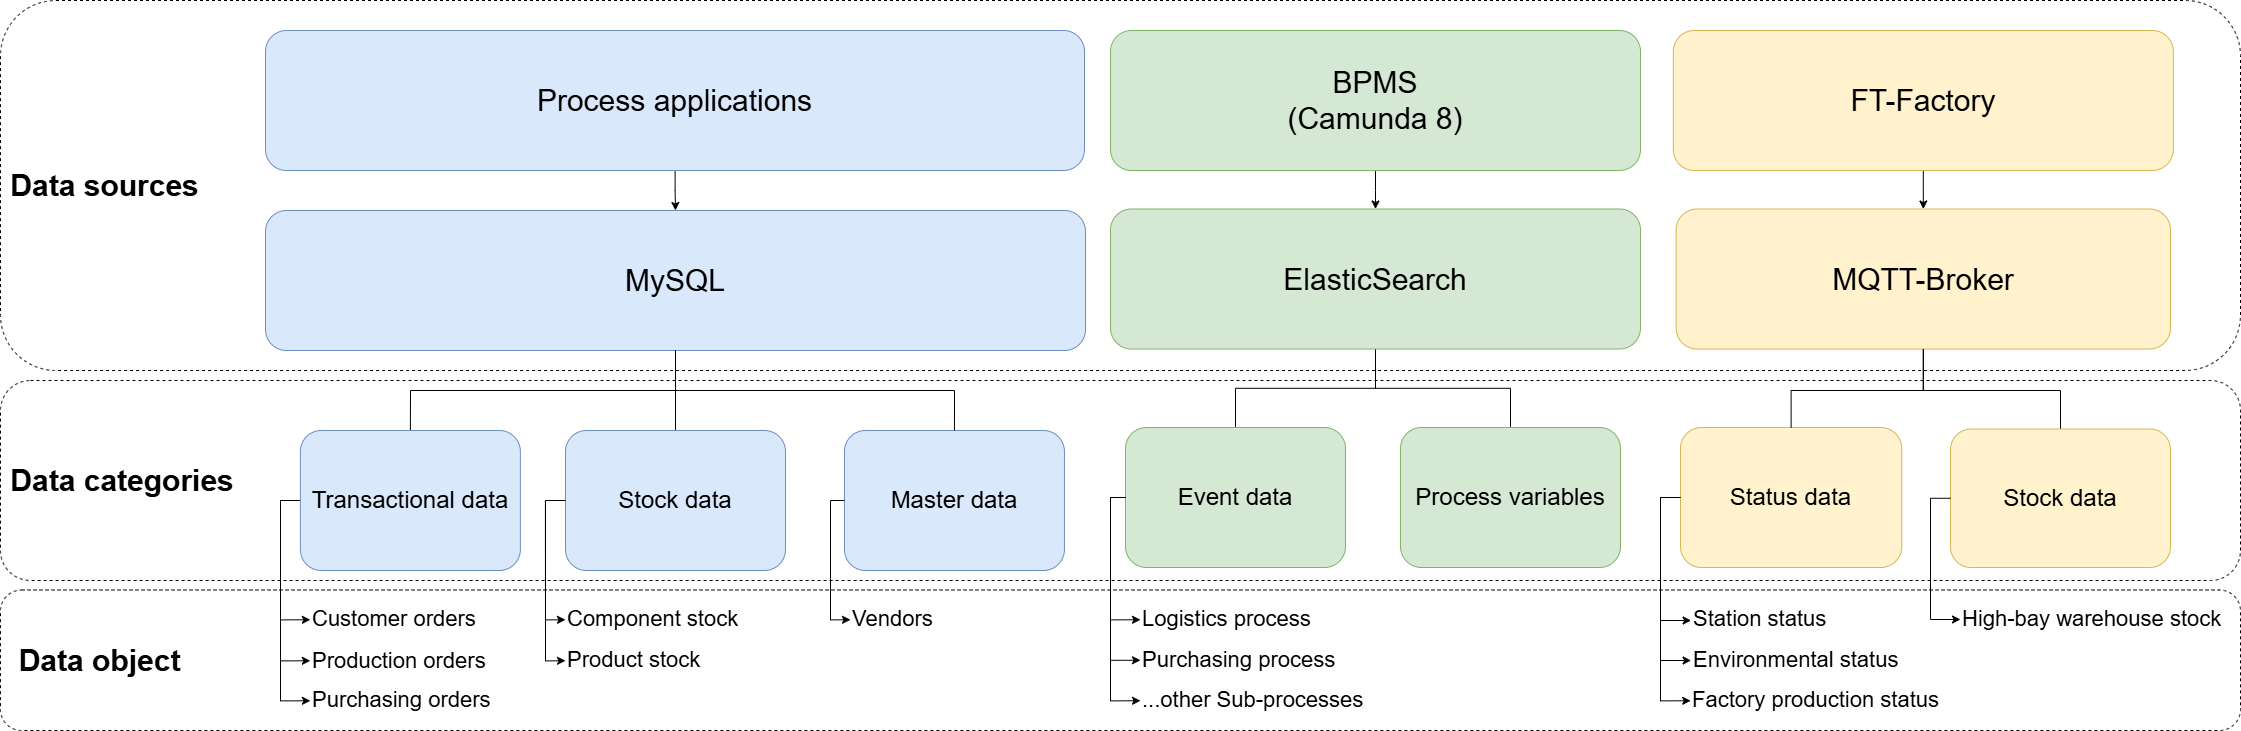
\includegraphics[keepaspectratio]{images/data_overview.png}}

}

\caption{\label{fig-data-overview}Data overview in the BPA Lab}

\end{figure}%

\section{The MySQL data model}\label{the-mysql-data-model}

The following diagram shows the concrete data model of the MySQL
database, including the entities and attributes of the current
implementation:

\begin{figure}

\centering{

\pandocbounded{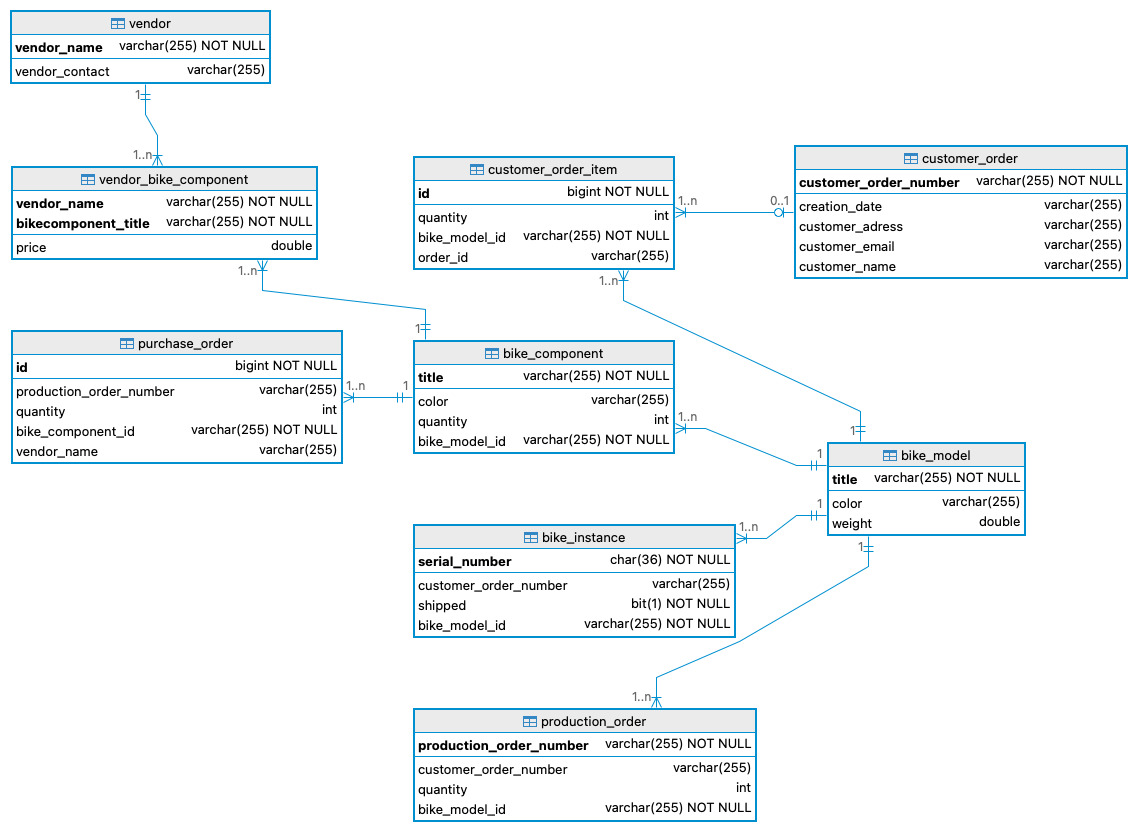
\includegraphics[keepaspectratio]{images/mysql_data_model.png}}

}

\caption{\label{fig-mysql}MySQL data model}

\end{figure}%

The database serves as the central store for:

\begin{itemize}
\tightlist
\item
  \textbf{Product master data} --- bicycle models and their components,
\item
  \textbf{Customer data} and delivery addresses,
\item
  \textbf{Stock levels} for components and finished goods,
\item
  \textbf{Orders} --- customer orders, production orders, purchase
  orders --- together with their status history,
\item
  \textbf{Vendor data}.
\end{itemize}

\section{Sample and master data}\label{sample-and-master-data}

Documentation and sample data of the Fischertechnik factory are
available in the
\href{https://github.com/BpaLabTHCologne/bpa_lab_docs/tree/main/Sample_data}{\texttt{Sample\_data}}
folder of the documentation repository. This data serves as:

\begin{itemize}
\tightlist
\item
  \textbf{initial master data} when setting up a new instance of the BPA
  Lab,
\item
  \textbf{test data} for developing new components,
\item
  a \textbf{demonstration baseline} for teaching sessions and
  presentations.
\end{itemize}

\section{Process data and the foundation for process
mining}\label{process-data-and-the-foundation-for-process-mining}

In addition to persistent master data, the running processes generate
substantial amounts of \textbf{process data}:

\begin{itemize}
\tightlist
\item
  \textbf{Camunda 8} stores process instance data, variables, tokens,
  and lifecycle events.
\item
  \textbf{MQTT messages} record the communication between job workers
  and controllers.
\item
  \textbf{Job worker logs} capture technical operations and exceptions.
\end{itemize}

This event data is the foundation for \textbf{process mining} --- a
central teaching and demonstration component of the BPA Lab. Process
mining allows students to:

\begin{itemize}
\tightlist
\item
  \textbf{discover} the actual flow of processes from event logs (and
  compare them to the modelled flow),
\item
  \textbf{check conformance} between modelled and actual behaviour,
\item
  \textbf{analyse performance} --- durations, bottlenecks, rework loops.
\end{itemize}

\begin{tcolorbox}[enhanced jigsaw, arc=.35mm, bottomrule=.15mm, bottomtitle=1mm, breakable, colback=white, colbacktitle=quarto-callout-tip-color!10!white, colframe=quarto-callout-tip-color-frame, coltitle=black, left=2mm, leftrule=.75mm, opacityback=0, opacitybacktitle=0.6, rightrule=.15mm, title=\textcolor{quarto-callout-tip-color}{\faLightbulb}\hspace{0.5em}{Extension idea}, titlerule=0mm, toprule=.15mm, toptitle=1mm]

For process-mining exercises, it is worth writing an event-log export
script that converts Camunda 8 data into the \textbf{XES} (eXtensible
Event Stream) format. This enables direct integration with tools such as
ProM, Disco, or PM4Py, and gives students a realistic data pipeline from
running process to analytical tool.

\end{tcolorbox}

\section{Data lifecycle and
analytics}\label{data-lifecycle-and-analytics}

Looking at the data lifecycle as a whole:

\begin{enumerate}
\def\labelenumi{\arabic{enumi}.}
\tightlist
\item
  \textbf{Master data} is loaded once when the lab is set up and updated
  when new products, customers, or vendors are added.
\item
  \textbf{Operational data} --- orders, stock movements, production
  orders --- is created continuously as processes run.
\item
  \textbf{Event data} is emitted by the workflow engine, the job
  workers, and the MQTT broker as side effects of process execution.
\item
  \textbf{Analytical data} is derived from the above by export and
  transformation pipelines, then fed into process-mining and BI tools.
\end{enumerate}

This layered view of data is itself a teaching opportunity: it mirrors
the classical separation of OLTP and OLAP systems that students will
encounter in industry.

\bookmarksetup{startatroot}

\chapter{Software Architecture}\label{software-architecture}

\begin{tcolorbox}[enhanced jigsaw, arc=.35mm, bottomrule=.15mm, bottomtitle=1mm, breakable, colback=white, colbacktitle=quarto-callout-note-color!10!white, colframe=quarto-callout-note-color-frame, coltitle=black, left=2mm, leftrule=.75mm, opacityback=0, opacitybacktitle=0.6, rightrule=.15mm, title=\textcolor{quarto-callout-note-color}{\faInfo}\hspace{0.5em}{Learning objectives}, titlerule=0mm, toprule=.15mm, toptitle=1mm]

After reading this chapter, you will be able to:

\begin{itemize}
\tightlist
\item
  name the high-level requirements that shaped the BPA Lab architecture,
\item
  describe the architecture using the C4 model,
\item
  relate individual architectural choices to the requirements that
  motivated them.
\end{itemize}

\end{tcolorbox}

\begin{tcolorbox}[enhanced jigsaw, arc=.35mm, bottomrule=.15mm, bottomtitle=1mm, breakable, colback=white, colbacktitle=quarto-callout-important-color!10!white, colframe=quarto-callout-important-color-frame, coltitle=black, left=2mm, leftrule=.75mm, opacityback=0, opacitybacktitle=0.6, rightrule=.15mm, title=\textcolor{quarto-callout-important-color}{\faExclamation}\hspace{0.5em}{Status}, titlerule=0mm, toprule=.15mm, toptitle=1mm]

The architecture is under continuous development. Several aspects are
still being discussed. This chapter captures the current state.

\end{tcolorbox}

\section{Requirements}\label{requirements}

The following high-level requirements were gathered at the very
beginning of the BPA Lab project (originally as part of a thesis
project). They served as the basis for the first software architecture
and remain the reference point against which architectural choices are
evaluated.

\subsection{R1 --- Independent operation of
components}\label{r1-independent-operation-of-components}

The individual components and processes should be able to run
independently of each other. Each process must be startable on its own,
without depending on a triggering instance from a higher layer.

\subsection{R2 --- Integration of external IT
systems}\label{r2-integration-of-external-it-systems}

The system must allow integration with existing IT components --- for
example with the web application used for order capture, or with tools
that flexibly extract data for process mining and analytics.

\subsection{R3 --- Clear and distinct
responsibilities}\label{r3-clear-and-distinct-responsibilities}

The responsibilities of individual components must be clearly defined
and demarcated from one another, so that the system remains
understandable as it grows.

\subsection{R4 --- Easy extensibility}\label{r4-easy-extensibility}

The system must be easy to extend with additional, self-developed
components.

\subsection{R5 --- Interchangeability and independent
evolution}\label{r5-interchangeability-and-independent-evolution}

Components must be developable, deployable, and replaceable
independently of one another.

\subsection{R6 --- Comprehensive and flexible process data
capture}\label{r6-comprehensive-and-flexible-process-data-capture}

Process data must be comprehensively capturable. It must be stored and
made flexibly available for a range of analytical use cases --- in
particular process mining.

\subsection{R7 --- User-friendliness (operator
perspective)}\label{r7-user-friendliness-operator-perspective}

The user interface must be intuitive and easy to understand, ensuring a
positive user experience for those interacting with the lab during
demonstrations and student sessions.

\subsection{R8 --- Easy installation and low infrastructure requirements
(developer
perspective)}\label{r8-easy-installation-and-low-infrastructure-requirements-developer-perspective}

The system must be easy to install. Students must be able to host their
own instances on standard laptops without specialised infrastructure.

\subsection{R9 --- Robustness}\label{r9-robustness}

The architecture must be robust. Failures must be minimised and reliable
functionality must be ensured under a wide range of operating
conditions.

\subsection{R10 --- Maintainability and
operation}\label{r10-maintainability-and-operation}

The system must be easy to maintain over its lifetime.

\section{Architecture in the C4
model}\label{architecture-in-the-c4-model}

The architecture is documented using the \textbf{C4 model} (Brown 2018)
--- a notation for describing software systems at different levels of
abstraction: Context, Container, Component, and Code. Note that
\emph{containers} in the C4 sense are \textbf{not} the same as Docker
containers.

\subsection{Context diagram}\label{context-diagram}

The context diagram shows the BPA Lab in relation to its users and
external systems.

\begin{figure}

\centering{

\pandocbounded{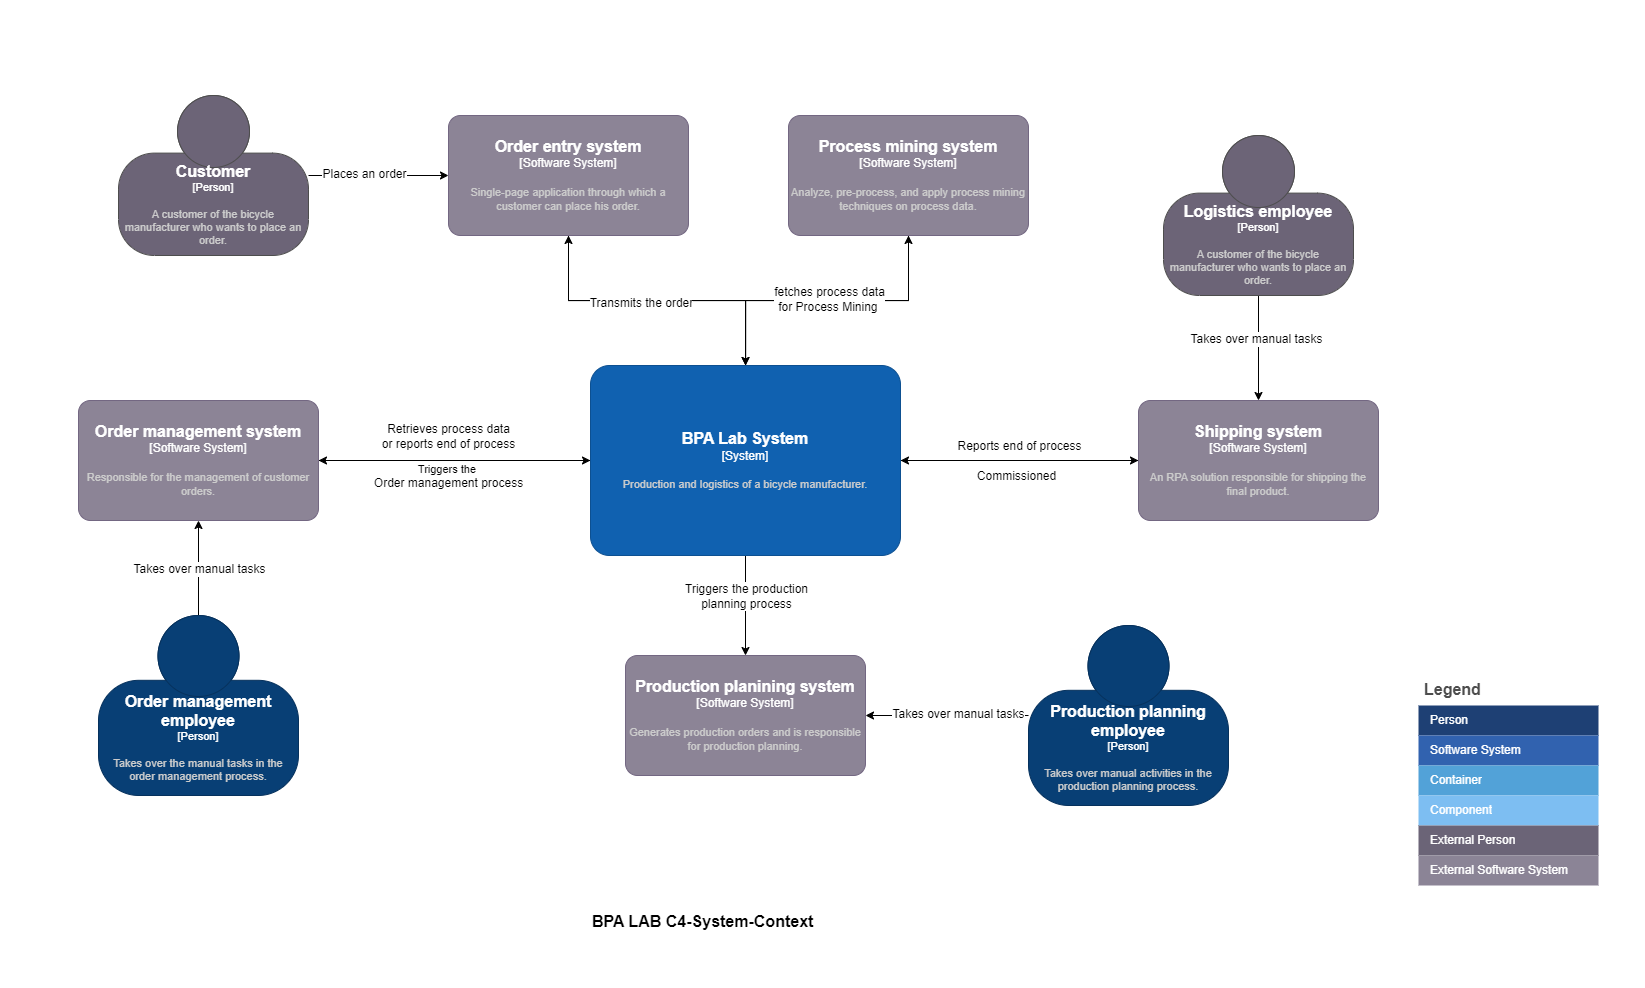
\includegraphics[keepaspectratio]{images/c4-contextDiagram.drawio.png}}

}

\caption{\label{fig-c4-context}C4 context diagram}

\end{figure}%

\subsection{Container diagram}\label{container-diagram}

The container diagram shows the main technical building blocks of the
BPA Lab and how they interact.

\begin{figure}

\centering{

\pandocbounded{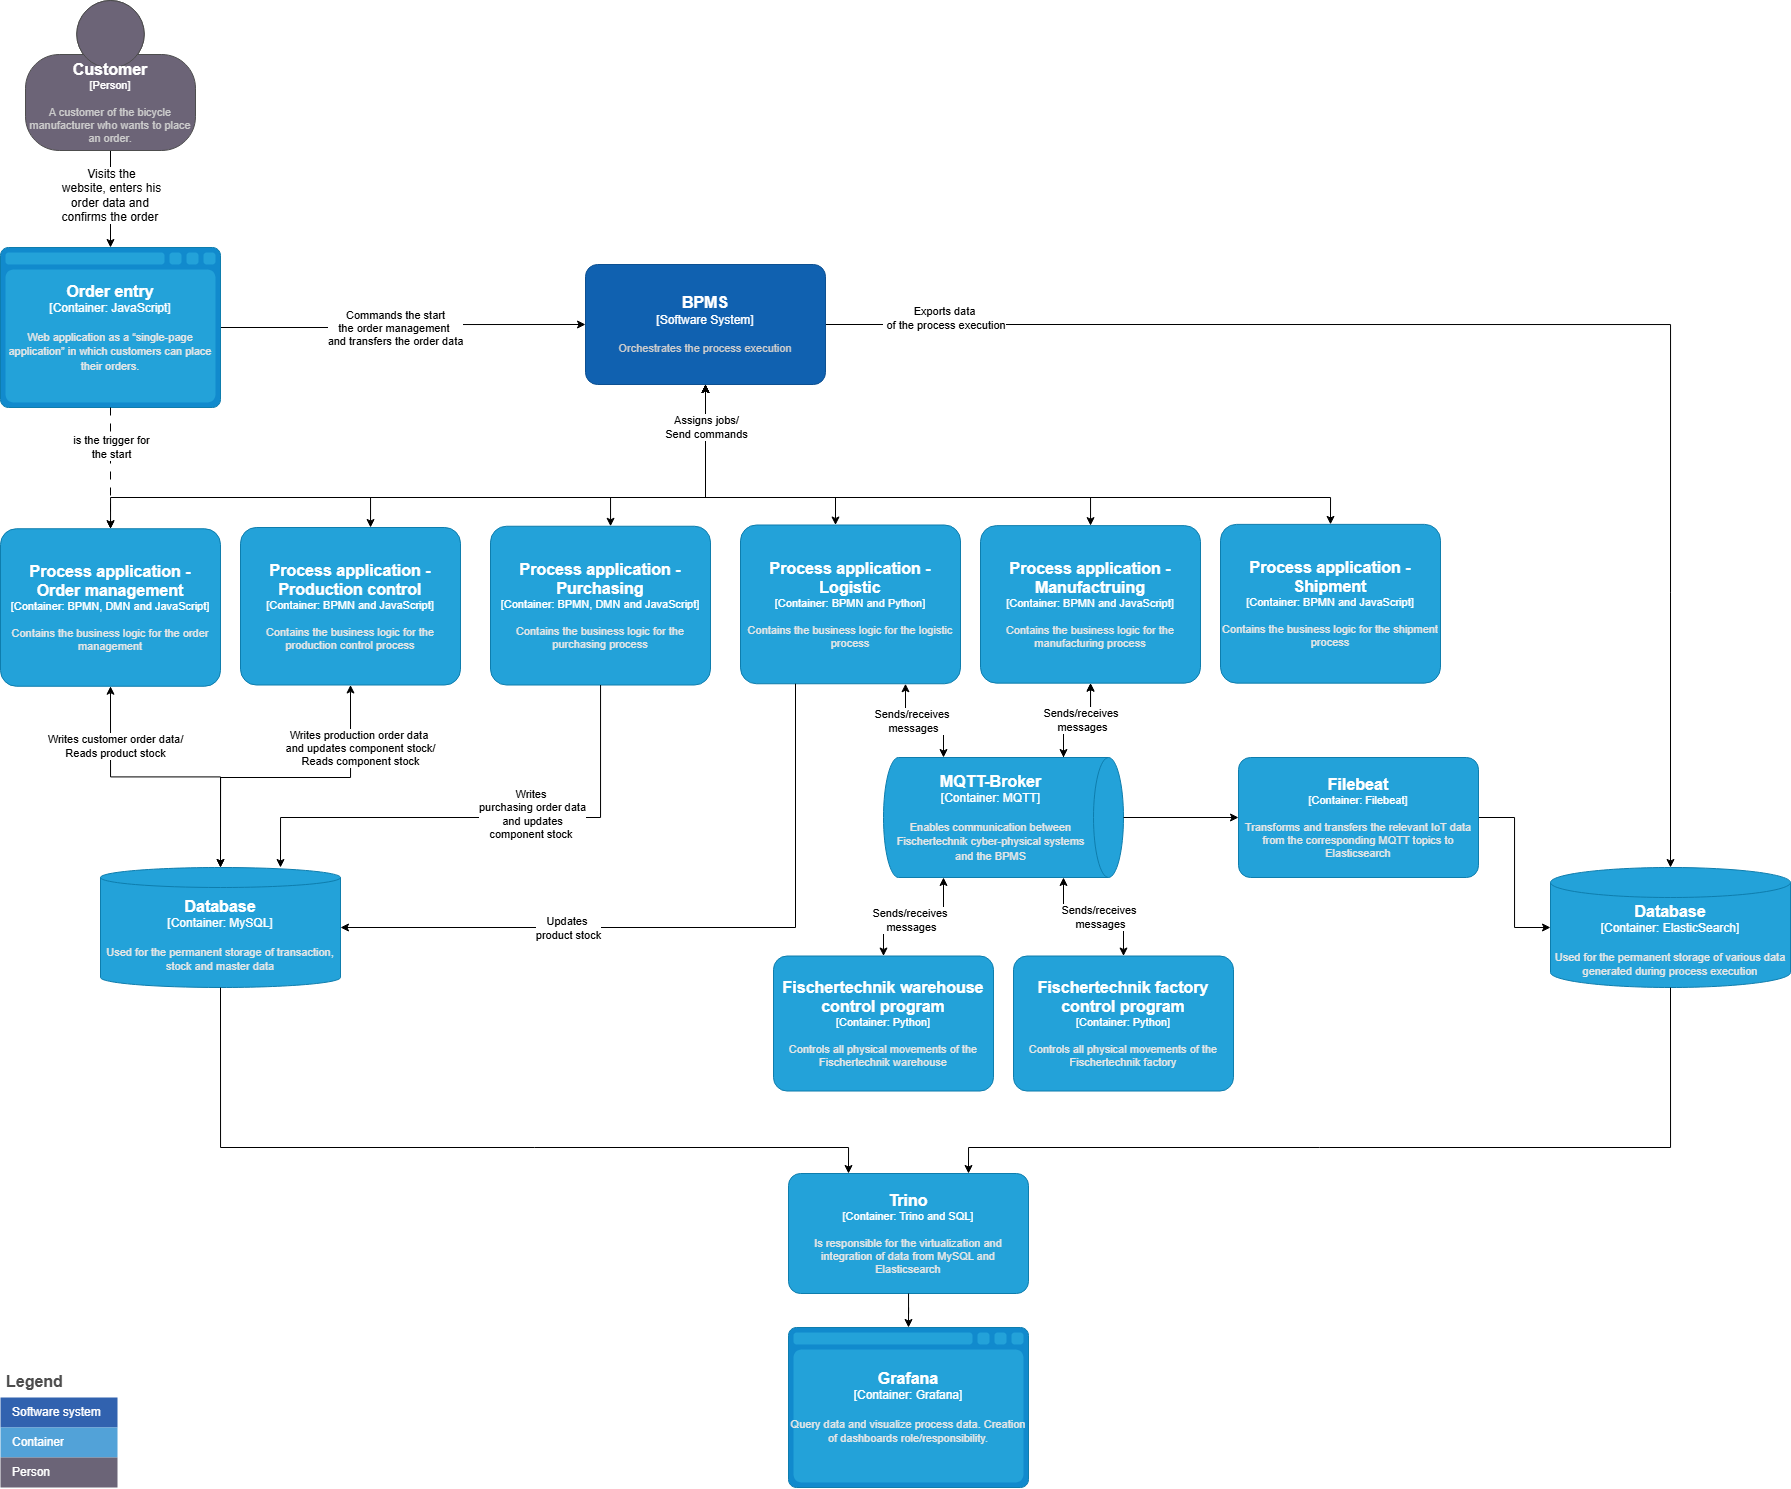
\includegraphics[keepaspectratio]{images/C4_System_Architecture.png}}

}

\caption{\label{fig-c4-container}C4 container diagram}

\end{figure}%

\section{Mapping requirements to
architecture}\label{mapping-requirements-to-architecture}

The following table illustrates how individual requirements are
addressed by architectural choices. It is not exhaustive --- but it
shows the line of reasoning from requirement to design.

{\def\LTcaptype{none} % do not increment counter
\begin{longtable}[]{@{}
  >{\raggedright\arraybackslash}p{(\linewidth - 2\tabcolsep) * \real{0.3710}}
  >{\raggedright\arraybackslash}p{(\linewidth - 2\tabcolsep) * \real{0.6290}}@{}}
\toprule\noalign{}
\begin{minipage}[b]{\linewidth}\raggedright
Requirement
\end{minipage} & \begin{minipage}[b]{\linewidth}\raggedright
Realisation in the architecture
\end{minipage} \\
\midrule\noalign{}
\endhead
\bottomrule\noalign{}
\endlastfoot
R1 --- Independent operation & Loose coupling via MQTT and gRPC;
self-contained job workers \\
R2 --- Integration of external systems & Standard protocols (REST, MQTT,
gRPC); Camunda connector concept \\
R3 --- Clear responsibilities & Domain-driven separation of job workers
and process models \\
R6 --- Process data capture & Camunda 8 as central event hub; MySQL for
operational data \\
R8 --- Easy installation & Docker Compose setup; self-managed Camunda 8
Core \\
R5/R9 --- Interchangeability / robustness & Asynchronous messaging;
clear interfaces between layers \\
\end{longtable}
}

\section{Going deeper}\label{going-deeper}

\begin{tcolorbox}[enhanced jigsaw, arc=.35mm, bottomrule=.15mm, bottomtitle=1mm, breakable, colback=white, colbacktitle=quarto-callout-tip-color!10!white, colframe=quarto-callout-tip-color-frame, coltitle=black, left=2mm, leftrule=.75mm, opacityback=0, opacitybacktitle=0.6, rightrule=.15mm, title=\textcolor{quarto-callout-tip-color}{\faLightbulb}\hspace{0.5em}{Further reading}, titlerule=0mm, toprule=.15mm, toptitle=1mm]

The original sources on the C4 model --- including examples, decision
records, and tools like \href{https://structurizr.com/}{Structurizr} ---
are available at \url{https://c4model.com/}. For a deeper dive into
Domain-Driven Design as the principle behind the modular separation, see
Evans (Evans 2003).

\end{tcolorbox}

\bookmarksetup{startatroot}

\chapter{Architecture Decisions}\label{architecture-decisions}

\begin{tcolorbox}[enhanced jigsaw, arc=.35mm, bottomrule=.15mm, bottomtitle=1mm, breakable, colback=white, colbacktitle=quarto-callout-note-color!10!white, colframe=quarto-callout-note-color-frame, coltitle=black, left=2mm, leftrule=.75mm, opacityback=0, opacitybacktitle=0.6, rightrule=.15mm, title=\textcolor{quarto-callout-note-color}{\faInfo}\hspace{0.5em}{Learning objectives}, titlerule=0mm, toprule=.15mm, toptitle=1mm]

After reading this chapter, you will be able to:

\begin{itemize}
\tightlist
\item
  explain the rationale behind the central architectural choices in the
  BPA Lab,
\item
  read and write lightweight Architecture Decision Records (ADRs),
\item
  reflect on typical trade-offs in BPM-centric architectures.
\end{itemize}

\end{tcolorbox}

This chapter records selected architecture questions raised during the
BPA Lab project, together with the corresponding decisions and
justifications. The list is \textbf{not exhaustive} and is updated as
the lab evolves.

Each decision follows a lightweight \textbf{ADR} (Architecture Decision
Record) schema: context, decision, and rationale are captured
succinctly.

\section{ADR-001 --- MQTT broker for job-worker--controller
communication}\label{adr-001-mqtt-broker-for-job-workercontroller-communication}

\textbf{Status:} Decided.

\textbf{Decision:} A MQTT broker is used for communication between
process applications (job workers) and controllers.

\textbf{Rationale:}

\begin{itemize}
\tightlist
\item
  decoupling of senders and receivers through the publish-subscribe
  pattern,
\item
  MQTT is a well-established standard protocol in the IoT space,
\item
  lightweight footprint, well suited to the hardware components in use.
\end{itemize}

\section{ADR-002 --- Message Send/Receive Tasks instead of Events for
inter-process
communication}\label{adr-002-message-sendreceive-tasks-instead-of-events-for-inter-process-communication}

\textbf{Status:} Decided.

\textbf{Decision:} Inter-process communication is modelled in BPMN using
\textbf{Message Send Tasks} and \textbf{Message Receive Tasks}, not
events.

\textbf{Rationale:}

\begin{itemize}
\tightlist
\item
  Tasks allow the use of \textbf{boundary events} --- for example to
  handle errors raised by job workers,
\item
  complex error paths and timeouts are easier to express.
\end{itemize}

\section{ADR-003 --- Messaging between processes and process
applications}\label{adr-003-messaging-between-processes-and-process-applications}

\textbf{Status:} Decided.

\textbf{Decision:} Communication between processes and process
applications is implemented using messages as well.

\textbf{Rationale:}

\begin{itemize}
\tightlist
\item
  a simple, uniform solution,
\item
  consistent with the communication pattern between process applications
  and process control.
\end{itemize}

\section{ADR-004 --- Camunda 8 self-managed with Docker Compose (Camunda
8
Core)}\label{adr-004-camunda-8-self-managed-with-docker-compose-camunda-8-core}

\textbf{Status:} Decided.

\textbf{Decision:} The self-managed variant of Camunda 8 is used in
combination with Docker Compose and Camunda 8 Core.

\textbf{Rationale:}

\begin{itemize}
\tightlist
\item
  avoids interferences between contributors during the development
  phase,
\item
  development and production-like environments are identical,
\item
  Kubernetes is intentionally not used --- the BPA Lab is not a
  production environment in the classical sense.
\end{itemize}

\textbf{Open question:} Performance with Docker and the resulting number
of containers needs to be verified as the system grows.

\section{ADR-005 --- Job worker for sending
emails}\label{adr-005-job-worker-for-sending-emails}

\textbf{Status:} Decided (reversible).

\textbf{Decision:} Email sending is implemented through a dedicated job
worker rather than via the SendGrid connector.

\textbf{Rationale:}

\begin{itemize}
\tightlist
\item
  issues encountered with the SendGrid connector at the time of the
  decision,
\item
  an existing solution was already in place in the project,
\item
  to be re-evaluated as Camunda 8 connectors continue to evolve.
\end{itemize}

\section{ADR-006 --- Job worker for database transactions; MySQL in a
Docker
container}\label{adr-006-job-worker-for-database-transactions-mysql-in-a-docker-container}

\textbf{Status:} Decided.

\textbf{Decision:} Database transactions are handled by a dedicated job
worker; the MySQL database runs in a Docker container.

\textbf{Rationale:}

\begin{itemize}
\tightlist
\item
  existing solution available in the project,
\item
  greater flexibility than the connectors available at the time of the
  decision.
\end{itemize}

\section{Reflection questions}\label{reflection-questions}

\begin{tcolorbox}[enhanced jigsaw, arc=.35mm, bottomrule=.15mm, bottomtitle=1mm, breakable, colback=white, colbacktitle=quarto-callout-tip-color!10!white, colframe=quarto-callout-tip-color-frame, coltitle=black, left=2mm, leftrule=.75mm, opacityback=0, opacitybacktitle=0.6, rightrule=.15mm, title=\textcolor{quarto-callout-tip-color}{\faLightbulb}\hspace{0.5em}{For your own consideration}, titlerule=0mm, toprule=.15mm, toptitle=1mm]

\begin{enumerate}
\def\labelenumi{\arabic{enumi}.}
\tightlist
\item
  ADR-001 selects MQTT. What \textbf{alternative protocols} could have
  been considered, and what trade-offs would they imply?
\item
  ADR-005 is explicitly marked as reversible. Which \textbf{criteria}
  would you use to decide whether to switch back to a connector-based
  solution?
\item
  ADR-004 deliberately avoids Kubernetes. Under which circumstances
  would that decision need to be revisited?
\end{enumerate}

\end{tcolorbox}

\cleardoublepage
\phantomsection
\addcontentsline{toc}{part}{Appendices}
\appendix

\chapter{Components and Sister
Repositories}\label{components-and-sister-repositories}

This appendix gives an overview of the repositories that together make
up the BPA Lab ecosystem, and lists the main hardware and software
components.

\section{Main repositories}\label{main-repositories}

\subsection{bpa\_lab\_docs}\label{bpa_lab_docs}

➡️ \url{https://github.com/BpaLabTHCologne/bpa_lab_docs}

\textbf{Role:} central documentation and architecture of the BPA Lab as
a demonstration factory. The source of the content in this book.

\textbf{Contains:}

\begin{itemize}
\tightlist
\item
  overarching architecture diagrams,
\item
  sample data of the Fischertechnik factory,
\item
  BPMN process models (overview),
\item
  C4 architecture diagrams,
\item
  updated graphics.
\end{itemize}

\subsection{bpa\_lab\_demonstration\_factory}\label{bpa_lab_demonstration_factory}

➡️
\url{https://github.com/BpaLabTHCologne/bpa_lab_demonstration_factory}

\textbf{Role:} current implementation of the demonstration factory. A
complete, runnable setup based on Docker.

\textbf{Contains:}

\begin{itemize}
\tightlist
\item
  self-managed Camunda 8 setup,
\item
  all job worker implementations (Java),
\item
  BPMN and DMN models of the business processes,
\item
  controller implementations (Python),
\item
  \texttt{docker-compose.yml} for local deployment.
\end{itemize}

\subsection{bpa\_lab\_student\_docs}\label{bpa_lab_student_docs}

➡️ \url{https://github.com/BpaLabTHCologne/bpa_lab_student_docs/wiki}

\textbf{Role:} documentation for student projects. Describes how
individual components (e.g.~the warehouse robot) can be used in
self-developed process implementations.

\textbf{Contains:}

\begin{itemize}
\tightlist
\item
  per-component how-to guides,
\item
  example projects,
\item
  notes on setting up subsystems independently.
\end{itemize}

\section{Hardware components}\label{hardware-components}

{\def\LTcaptype{none} % do not increment counter
\begin{longtable}[]{@{}
  >{\raggedright\arraybackslash}p{(\linewidth - 4\tabcolsep) * \real{0.3390}}
  >{\raggedright\arraybackslash}p{(\linewidth - 4\tabcolsep) * \real{0.4576}}
  >{\raggedright\arraybackslash}p{(\linewidth - 4\tabcolsep) * \real{0.2034}}@{}}
\toprule\noalign{}
\begin{minipage}[b]{\linewidth}\raggedright
Component
\end{minipage} & \begin{minipage}[b]{\linewidth}\raggedright
Purpose
\end{minipage} & \begin{minipage}[b]{\linewidth}\raggedright
Control
\end{minipage} \\
\midrule\noalign{}
\endhead
\bottomrule\noalign{}
\endlastfoot
Fischertechnik Industry 4.0 factory & Goods receipt and manufacturing &
Python controller, MQTT \\
Fischertechnik warehouse robot & Storage and retrieval in the
distribution warehouse & Python controller, MQTT \\
IoT devices & Sensor data and supplementary telemetry & Python
controller, MQTT \\
\end{longtable}
}

\section{Software components}\label{software-components}

{\def\LTcaptype{none} % do not increment counter
\begin{longtable}[]{@{}
  >{\raggedright\arraybackslash}p{(\linewidth - 4\tabcolsep) * \real{0.2476}}
  >{\raggedright\arraybackslash}p{(\linewidth - 4\tabcolsep) * \real{0.2762}}
  >{\raggedright\arraybackslash}p{(\linewidth - 4\tabcolsep) * \real{0.4762}}@{}}
\toprule\noalign{}
\begin{minipage}[b]{\linewidth}\raggedright
Component
\end{minipage} & \begin{minipage}[b]{\linewidth}\raggedright
Technology
\end{minipage} & \begin{minipage}[b]{\linewidth}\raggedright
Main responsibility
\end{minipage} \\
\midrule\noalign{}
\endhead
\bottomrule\noalign{}
\endlastfoot
Camunda 8 (self-managed) & BPMS, based on Zeebe & Workflow engine and
process orchestration \\
Job workers & Java, gRPC & Execution of service tasks \\
Controllers & Python & Hardware control \\
MQTT broker & e.g.~Mosquitto & Asynchronous communication \\
MySQL & Relational database & Master data and stock data \\
Web application & Frontend & Order capture and user interaction \\
Openrouteservice & External API & Distance and routing calculation in
the shipment process \\
\end{longtable}
}

\section{Further reading}\label{further-reading-1}

As the BPA Lab is under continuous development, it is always worth
checking the respective repository READMEs for the most current
information.

\chapter{Glossary}\label{glossary}

This appendix explains the technical terms used throughout the book.

\begin{description}
\tightlist
\item[\textbf{ADR (Architecture Decision Record)}]
Lightweight documentation format for recording architectural decisions
in a structured way --- context, decision, and rationale.
\item[\textbf{BPA (Business Process Automation)}]
The use of technology to automate the execution of business processes.
\item[\textbf{BPMN (Business Process Model and Notation)}]
A standard of the Object Management Group (OMG) for graphical modelling
of business processes. Current version: 2.0.2 (Object Management Group
2014).
\item[\textbf{BPMS (Business Process Management System)}]
A platform for modelling, executing, monitoring, and optimising business
processes. The BPA Lab uses Camunda 8.
\item[\textbf{Camunda 8}]
A cloud-native BPMS built around the Zeebe workflow engine. The BPA Lab
uses the \emph{self-managed} variant (Camunda Services GmbH 2026).
\item[\textbf{Controller}]
In the BPA Lab, a software component that directly controls hardware
(Fischertechnik components, IoT devices). Predominantly implemented in
Python.
\item[\textbf{C4 model}]
A notation for visualising software architecture at four levels of
abstraction: Context, Container, Component, Code. Introduced by Simon
Brown --- \url{https://c4model.com/} (Brown 2018).
\item[\textbf{DDD (Domain-Driven Design)}]
An approach to software development that places the business domain at
the centre. The guiding principle for the modular decomposition of the
BPA Lab (Evans 2003).
\item[\textbf{DMN (Decision Model and Notation)}]
An OMG standard for modelling business decisions (Object Management
Group 2024). Supported in Camunda 8 as a complement to BPMN.
\item[\textbf{End-to-end process}]
A business process viewed from its triggering event through to its final
business outcome --- in the BPA Lab, from the arrival of a customer
order to the delivery of a bicycle.
\item[\textbf{Fischertechnik Industry 4.0 factory}]
A modular model of an Industry-4.0 factory by Fischertechnik. In the BPA
Lab, it serves as the physical demonstration system.
\item[\textbf{gRPC}]
A high-performance Remote Procedure Call framework originated at Google.
In the BPA Lab, Camunda 8 uses gRPC to communicate with job workers.
\item[\textbf{Happy path}]
The path through a process in which no errors, exceptions, or edge cases
occur.
\item[\textbf{IoT (Internet of Things)}]
The networking of physical devices with the internet and with each
other.
\item[\textbf{Job worker}]
In Camunda 8, an external application that picks up service tasks from
the workflow and executes them. In the BPA Lab, job workers are
implemented in Java.
\item[\textbf{MQTT (Message Queuing Telemetry Transport)}]
A lightweight publish-subscribe protocol widely used in the IoT space.
In the BPA Lab, MQTT is the communication protocol between job workers
and controllers.
\item[\textbf{Openrouteservice}]
A public API for routing and distance calculation based on OpenStreetMap
data. Used in the BPA Lab's shipment process.
\item[\textbf{Process mining}]
Data-driven analysis of business processes based on event logs from
information systems. A central teaching and demonstration component in
the BPA Lab (Aalst 2016).
\item[\textbf{Process application}]
In the BPA Lab, a logical grouping of job workers and process models
belonging to one business domain (e.g.~\emph{Order Management}).
\item[\textbf{Production order}]
An order to manufacture a specific product. In the BPA Lab, one
production order is created per product line in a customer order.
\item[\textbf{RPA (Robotic Process Automation)}]
A technology to automate manual, repetitive tasks in existing
applications via their user interface.
\item[\textbf{Workflow engine}]
A software component that executes process models (e.g.~expressed in
BPMN), manages the state of process instances, and distributes work to
humans or job workers.
\item[\textbf{XES (eXtensible Event Stream)}]
An IEEE standard for event logs in process mining --- a format for the
exchange of process event data between systems.
\end{description}

\chapter{References}\label{references}

\protect\phantomsection\label{refs}
\begin{CSLReferences}{1}{1}
\bibitem[\citeproctext]{ref-vanderaalst2016processmining}
Aalst, Wil M. P. van der. 2016. \emph{Process Mining: Data Science in
Action}. 2nd ed. Springer.
\url{https://doi.org/10.1007/978-3-662-49851-4}.

\bibitem[\citeproctext]{ref-brown2018c4}
Brown, Simon. 2018. \emph{The {C4} Model for Visualising Software
Architecture}. Leanpub. \url{https://c4model.com/}.

\bibitem[\citeproctext]{ref-camunda8-docs}
Camunda Services GmbH. 2026. \emph{Camunda 8 Documentation}.
\url{https://docs.camunda.io/}.

\bibitem[\citeproctext]{ref-evans2003ddd}
Evans, Eric. 2003. \emph{Domain-Driven Design: Tackling Complexity in
the Heart of Software}. Addison-Wesley.

\bibitem[\citeproctext]{ref-omg-bpmn}
Object Management Group. 2014. \emph{Business Process Model and Notation
({BPMN}), Version 2.0.2}. \url{https://www.omg.org/spec/BPMN/}.

\bibitem[\citeproctext]{ref-omg-dmn}
Object Management Group. 2024. \emph{Decision Model and Notation
({DMN})}. \url{https://www.omg.org/spec/DMN/}.

\end{CSLReferences}


\backmatter


\end{document}
